% % Chapter 2: XAFS Simulations
% % Chapter 2: XANES
% \textit{In this section, I can write about XANES to a super in-depth extent, and likely the bulk of this chapter will be about FEFF and FDMNES theoretical calculations}
% \section{Maybe derivation of EXAFS Equation}
% \section{FEFF vs. FDMNES Approaches}
% \section{Theoretical XANES Calculations}
% -------------------------------------------------------------

Before making any predictions, neural networks must first be trained on a large quantity of data. In the context of this thesis, to teach our neural network to predict the mean squared displacement (MSD) from XANES, we must first assemble a collection of training data comprised of XANES spectra, each labeled with a known MSD. Gathering such a large quantity of high-quality experimental data would be impractically time-intensitive and expensive. Instead, simulations provide a practical alternative, though even simulating each possible disordered structure is time-intensive. This process has been standard practice in theoretical XAFS work and discussed in section \ref{sec:traditional-disorder}. 

We have conducted a significant amount of work in developing a new approach for simulating disordered XANES spectra. A discussion on the development of this new, statistical approach is presented in sections \ref{sec:start-disorder}--\ref{sec:end-disorder}. This new process is based on the statistical averaging of non-disordered structures. Instead of simulating hundreds of defined, disordered structures, we run many XANES simulations of simple, non-disordered structures and generate the disordered spectra via purposeful statistical averaging. In sections \ref{sec:start-disorder}--\ref{sec:end-disorder}, we explain this statistical weighting process in-depth, beginning with the creation of simple, non-disordered spectra for the FEFF input files and culminating in the creation of many possible disordered spectra with known MSDs. Finally, the efficacy and limitations of this approach are discussed in section \ref{sec:pa-feff-vs-gaussian-feff}.

\section{Traditional Particle-Averaged Simulations} 
\label{sec:traditional-disorder}
We refer to the traditional method for running FEFF simulations as particle-averaged FEFF. The simulation software, FEFF9 \cite{feff-citation}, only simulates the absorption spectrum for one absorber at a time. For this project, we are interested, at first, in simulating bulk Au. Accordingly, we attempt to remove the surface effects on the spectrum by simulating the absorption of only the first shell atoms and averaging (arithmetic mean) the results. This way, the first shell absorber atoms are surrounded by bulk structure, allowing FEFF to minimize the contribution of surface effects which affect the potential and multiple scatterings differently than the bulk. We made the decision to first simulate bulk Au in order to reduce the number of confounding variables; if the statistical averaging technique works for simulating disordered bulk structures, the next stage would be to expand the process to nanoparticles. 

Simulating absorption spectra via FEFF requires the creation of FEFF input files which include various user-defined parameters and the Euclidean coordinates of the structure. Determining how to create these structures is a project in and of itself. The approach taken for this experiment was to start with the perfectly ordered crystal of Au atoms. Then, for each structure, each individual atom is shifted by a random distance in a random direction. For each atom (in a given structure), the direction to be shifted is chosen from a uniform distribution, whereas the distance by which to shift the atom from its original location is chosen from a Gaussian. The standard deviation of the Gaussian from which the shifted distance is drawn differs from structure to structure. Thus, with a narrow width Gaussian, the shifted distances on average tend to be smaller than for a gaussian with a large width. Therefore, structures with small MSDs tend to be created when the width of the Gaussian for shift distances is narrow, whereas high MSD structures tend to be created when the width of the Gaussian is wide. The code for this script can be found in Appendix \ref{app:gen-train-data}.

Absorption simulation software is far from perfect, especially for XANES. There are different ways to treat the electronic potential and Fermi energies of the structure, none of which work best in all circumstances. FEFF works by simulating the green's function. A more in-depth description of how FEFF works can be found in Appendix B. FEFF includes many user-defined parameters which can be tweaked to alter the resulting function. By comparing the resulting FEFF spectrum to a reference experimental spectrum, an exhaustive grid search (parameter sweep) can be run to determine the best FEFF parameters for simulating a given structure. Each FEFF input file was run with the following paramters:

\vspace{2em}
\begin{minipage}{\linewidth}
	% Each FEFF input file is run with the following parameters: 
	\begin{Verbatim}[samepage=true, numbers=left]
		SCF 4.6 0 30 .5 1
		EDGE    L3
		EXCHANGE    5   0.2 0.5
		S02 1.
		XANES   3.7 0.05    0.1
		FMS 7
	
		POTENTIALS
		0	79	Au	-1	-1	0.
		1	79	Au	-1	-1	0.
	\end{Verbatim}
	~
	\end{minipage}
\noindent An explanation for the meaning behind these parameters can be found in Appendix section \ref{app:feff-cards}.

While particle averaging is the traditional method for simulating XANES via FEFF, the method is computationally intensive for large structures with many absorbers. One advantage of developing a statistical averaging method would be the ability to create an infinite number of disordered XANES spectra from a limited number of simulations. For particle averaging, to create 1000 disordered structures requires 13,000 simulations\footnote{1000 structures $ \times $ 13 absorbers per structure = 13,000 simulations}, a process that necessitates several days of computation time on a dedicated distributed computing cluster.



\begin{figure}[h!]
	\centering
	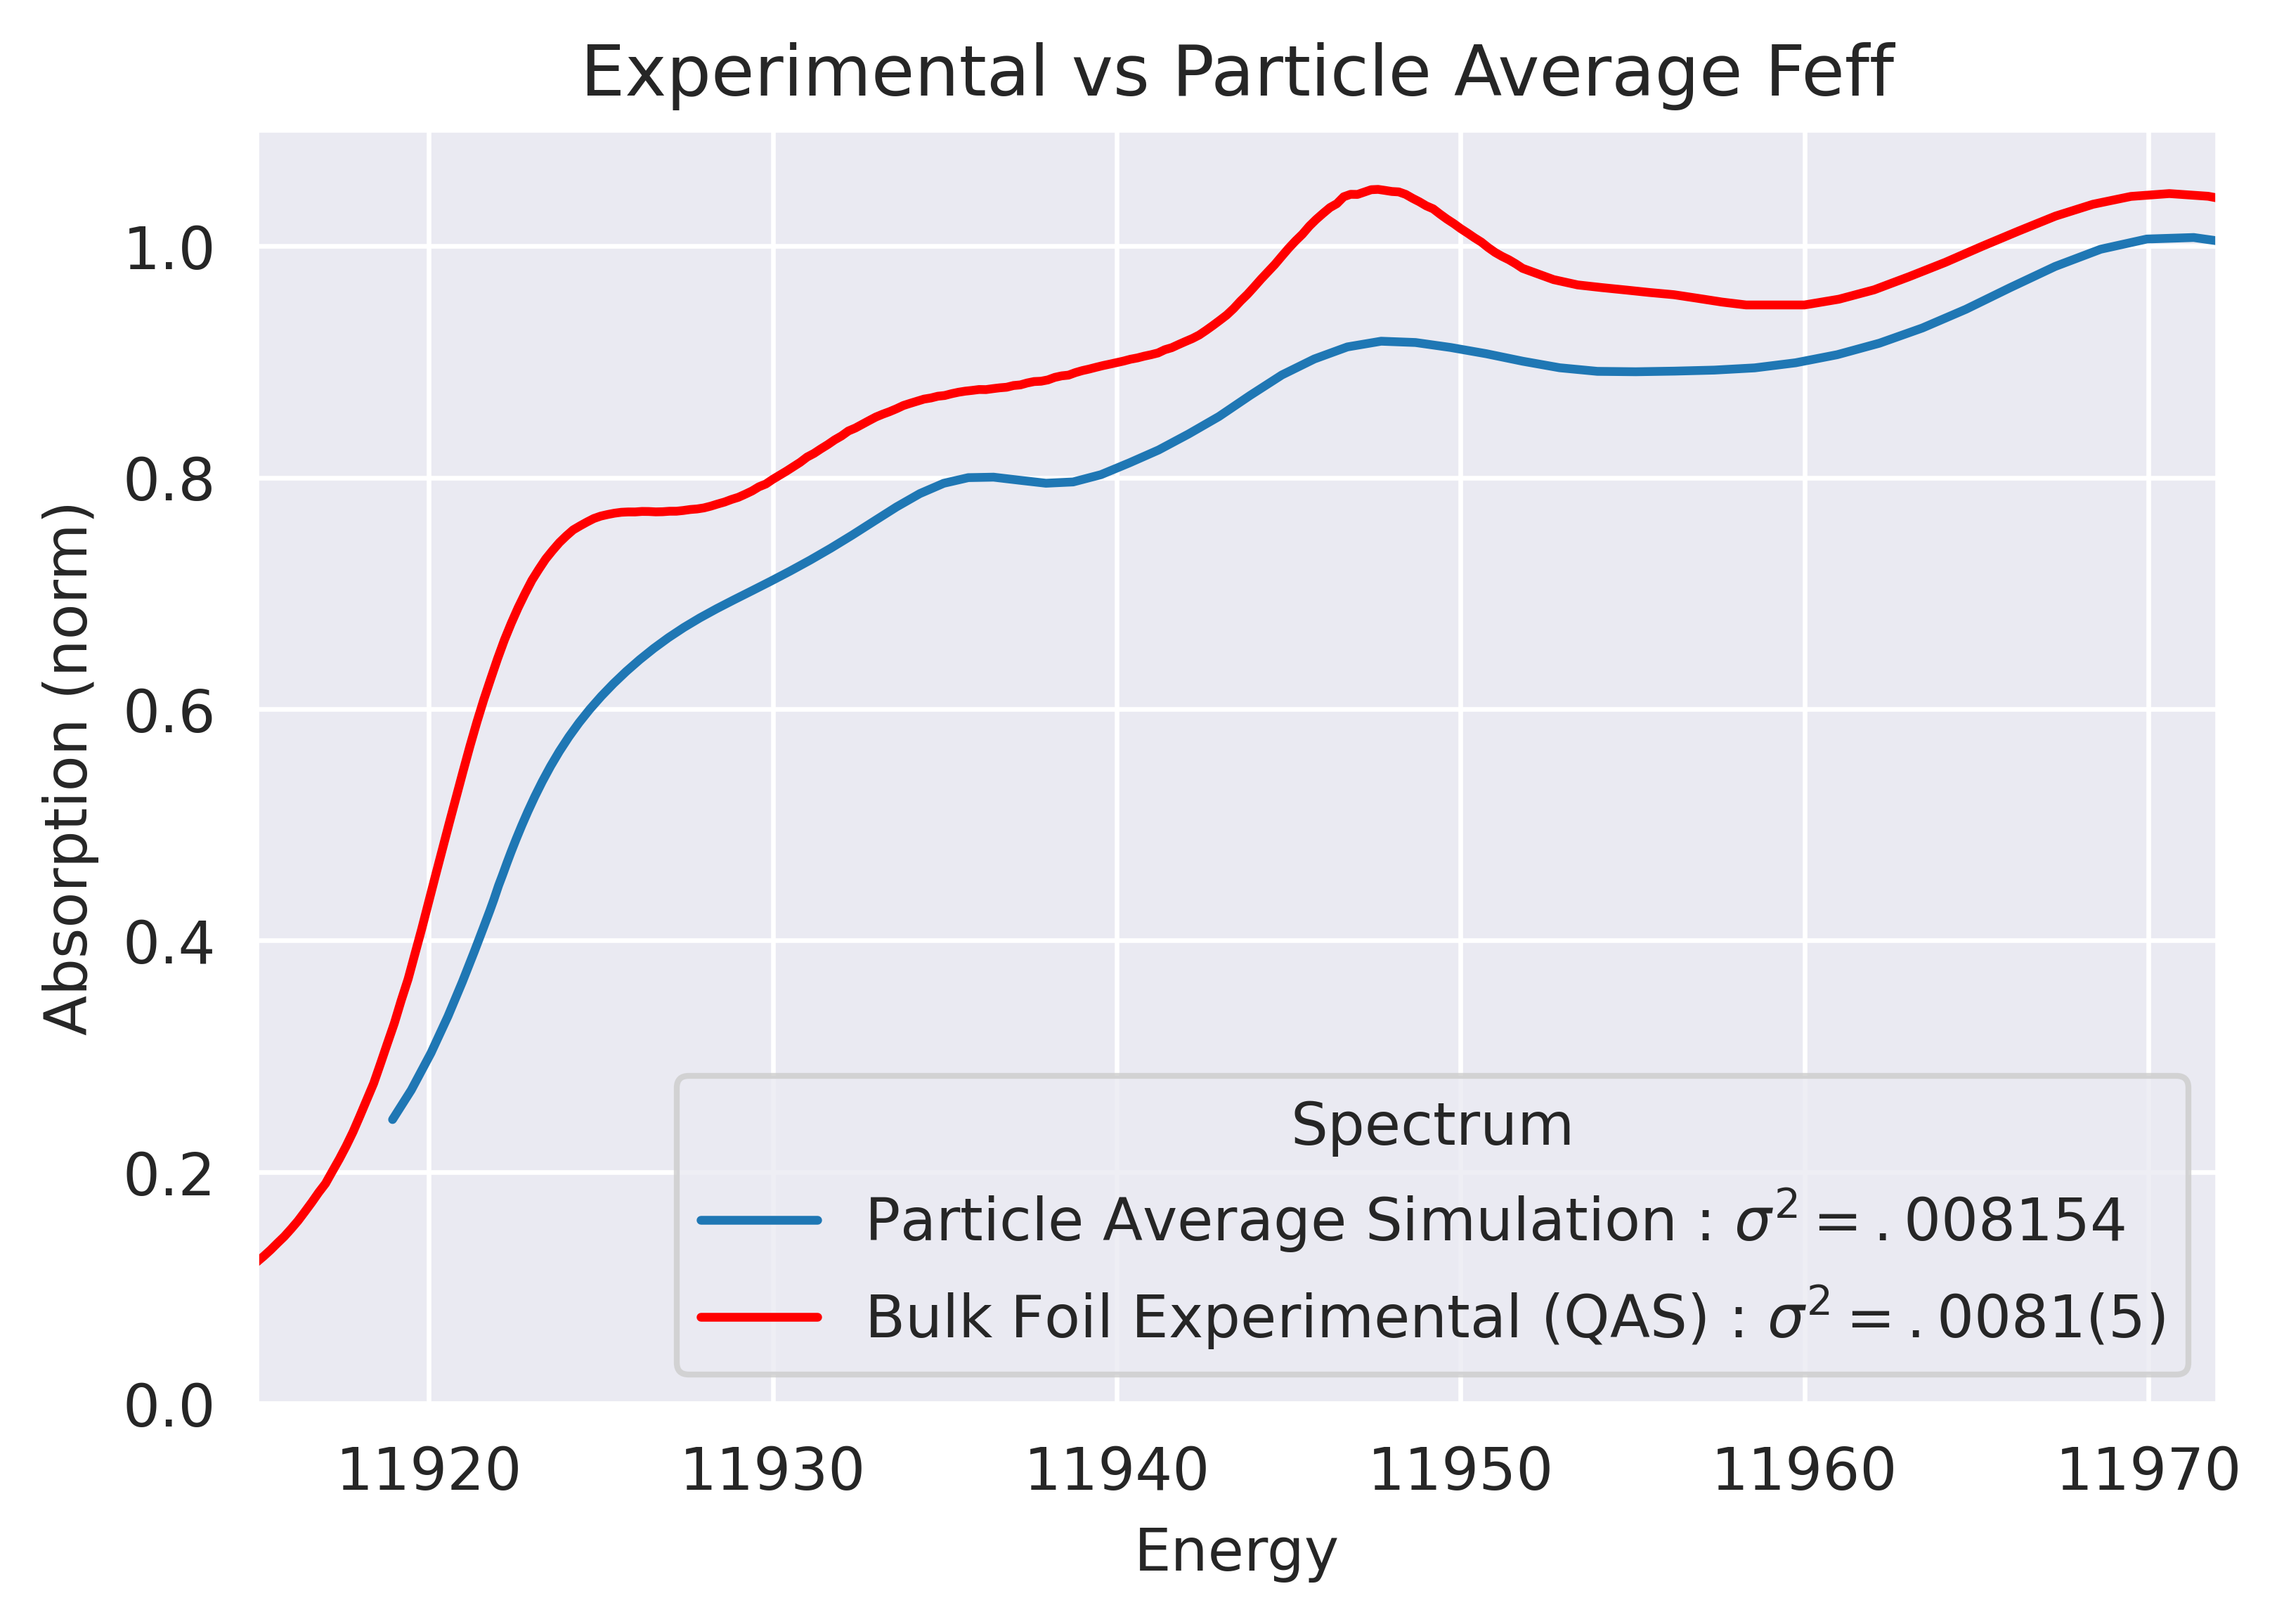
\includegraphics[width=.7\linewidth]{Chapters/Figures/Bulk_experimental_vs_pa_comparison.png}
	\caption[Simulation vs. Experimental 3]{Comparing the bulk foil (red) measurement to a simulated large, bulk-like nanoparticle with the same disorder. The FEFF-simulated version underestimates the magnitude of the oscillations at lower energies.}
	\label{fig:avg-experimental-vs-simulation2}
\end{figure}

\section{Statistical-Averaged Simulations}
To expedite the process of simulating XANES spectra of disordered structures, we have developed a new methodology build on a statistical averaging of a few easily simulated structures.

\subsection{Generating Distortion Not Disorder} \label{sec:start-disorder}
Instead of creating structures with a range of \textit{disorder}, we begin by generating structures with a range of \textit{distortion}. Whereas \textit{disorder} refers to a stochastic displacement of atoms from their original positions characterized by MSD and the width $ \sigma^2 $ of a radial distribution function, \textit{distortion} refers to isotropic expansion or contraction of the subject. Equivalently, we define distortion as a radial shift in all atomic positions away from (or towards) the center atomic absorber.

% Figure created in distortion-visualizations.ipynb 
\begin{figure}[h]
	\centering
	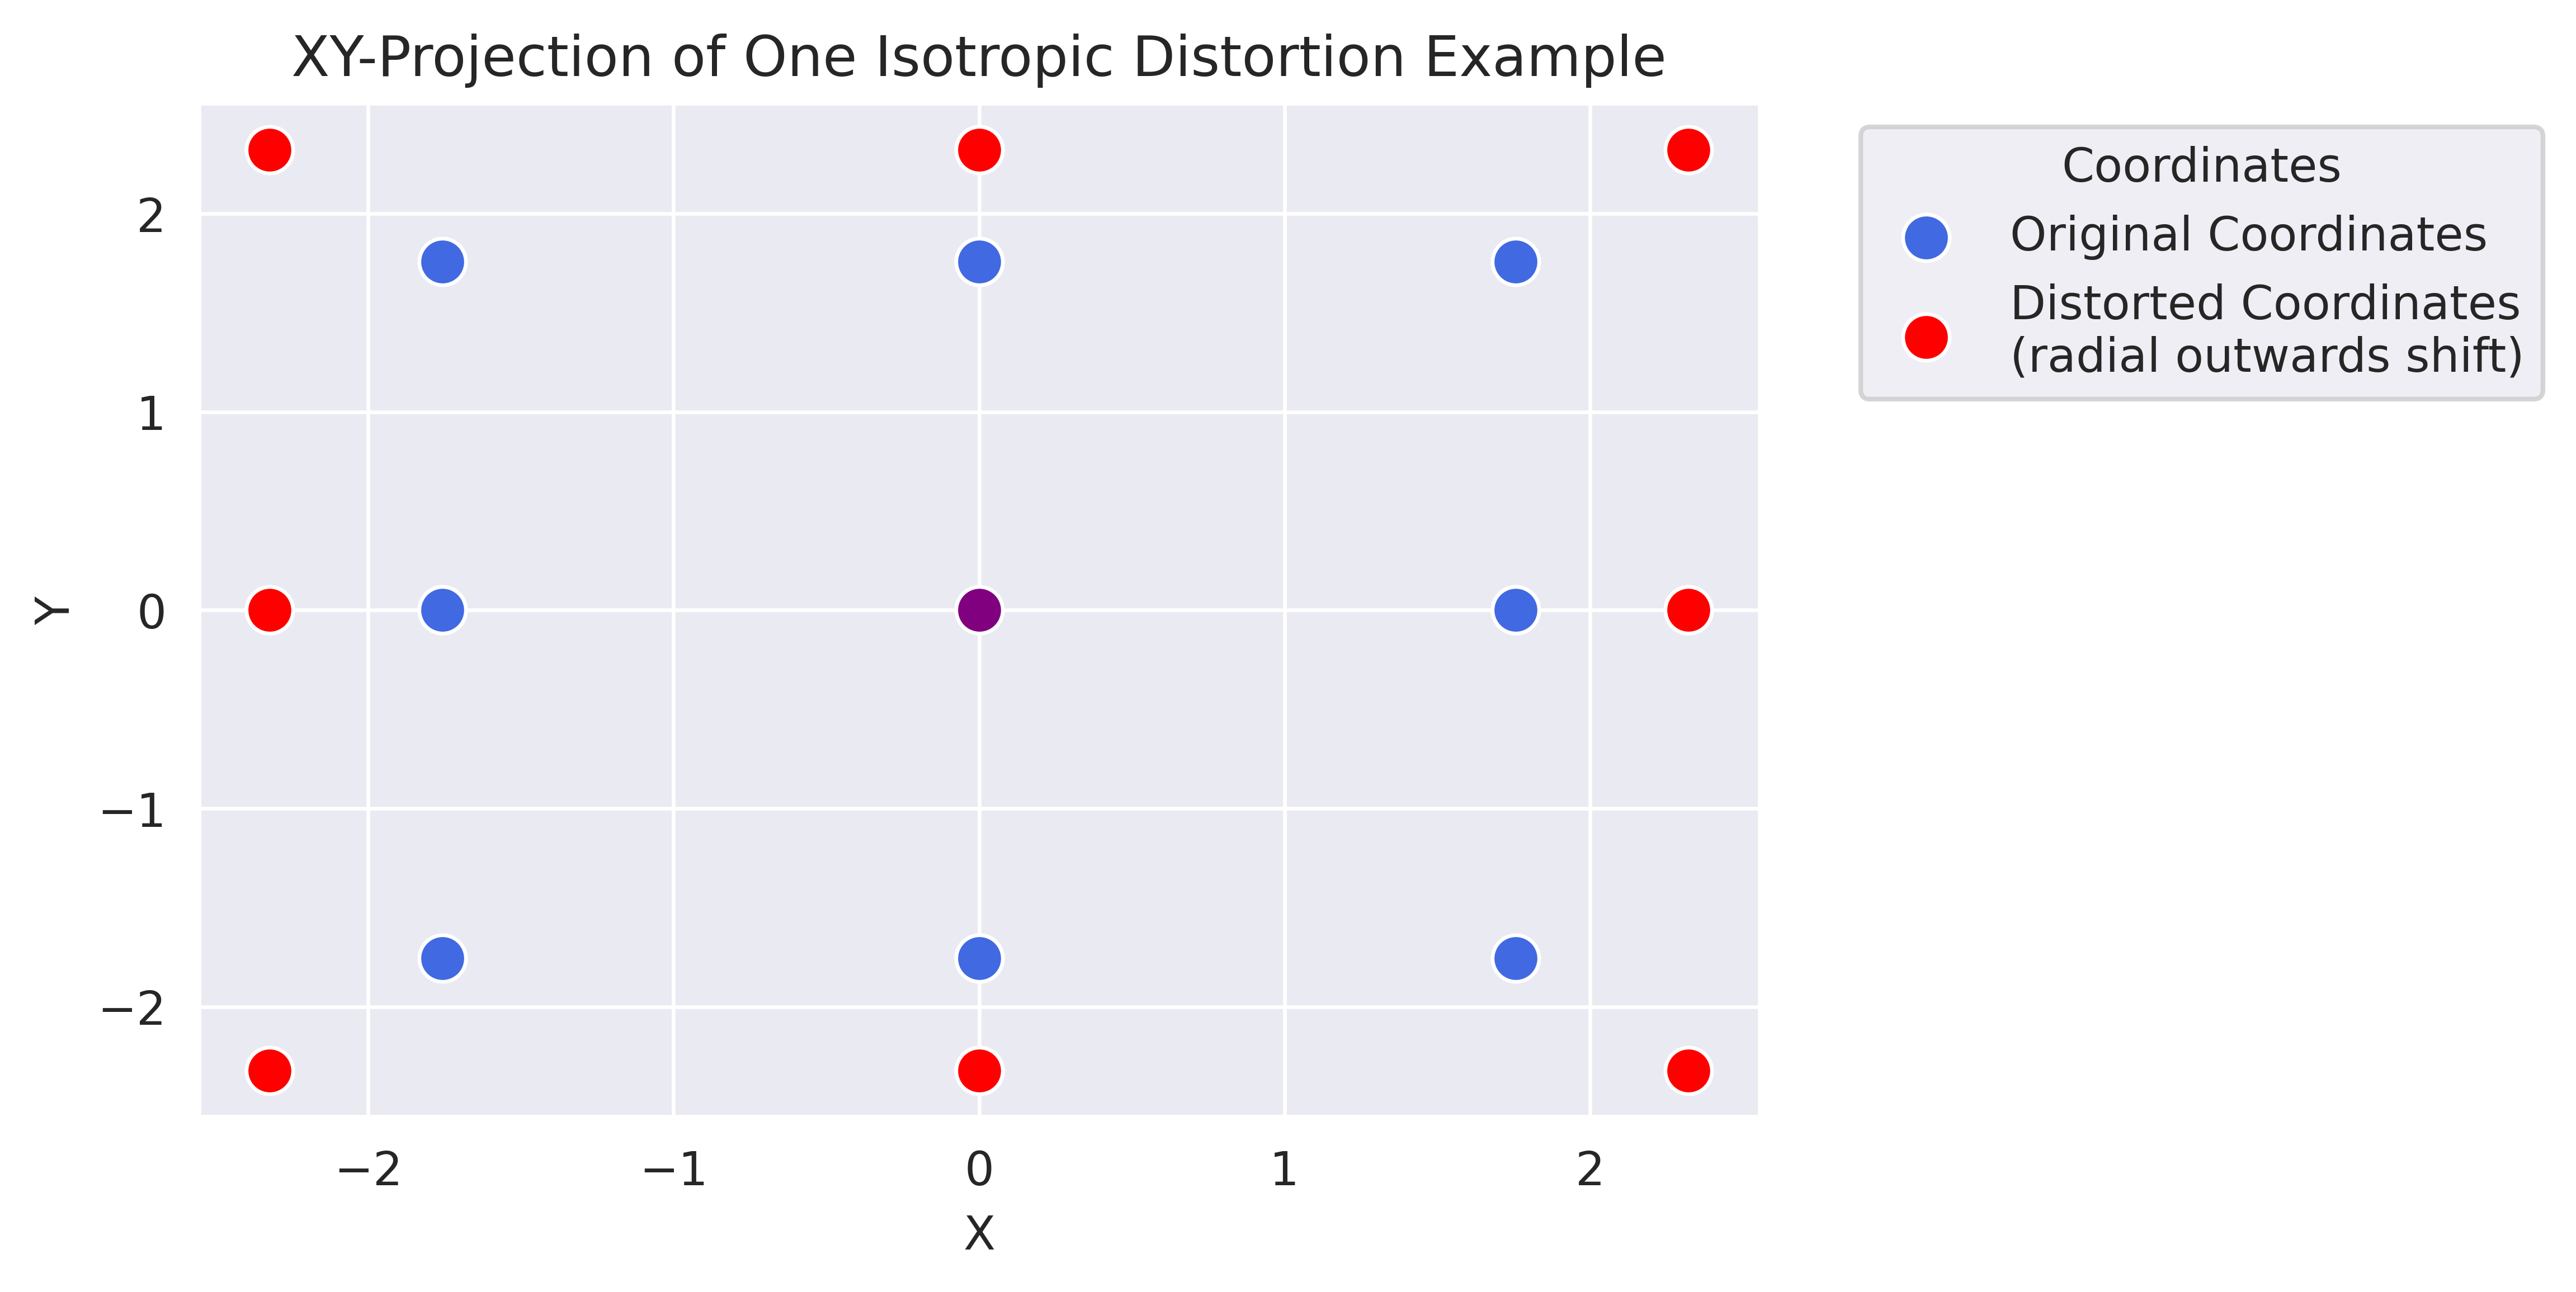
\includegraphics[width=\linewidth]{Chapters/Figures/2d_distortion_example.png}
	\caption[2D Distortion]{Each point represents an atom of first 12 nearest neighbors of a Au cluster projected onto the $xy$\nobreakdash-plane. The four corner points actually represent two atoms because of the projection. The blue atoms represent the original coordinates, and the red atoms represent the radially shifted coordinates. The center absorber atom is purple since its original position is the same as its distorted position.}
	\label{fig:2d-distortion}
\end{figure}

A 2-dimensional projection of this isotropic distortion is presented in Figure \ref{fig:2d-distortion}. Though the figure only shows the $xy$\nobreakdash-plane projection of the first 12 nearest neighbors, the actual structure consists of either 55 atoms to simulate a nanoparticles, or the first four shells (561 atoms) to simulate bulk materials. Both structures were created with a lattice constant of 4.0782~\AA~to match that of bulk Au \cite{gold-a-value-data}. In reality, the nearest-neighbor distances for Au nanoparticles are likely smaller than for the bulk structure; this can be accounted for later on in the averaging process since the original coordinates will only be one structure out of many. The important part is that the BCC crystal structure is correct. 

We generate a total of 91 FEFF input files with different levels of distortion. Each file contains the same center absorber located at $(0,0,0)$ with all the Euclidean distances from the center expanded or contracted radially. All the first shell atomic coordinates are shifted on the range of $ -0.45 $~\AA~to~$ +0.45 $~\AA~in increments of $ 0.01 $~\AA. For example, the FEFF input file with the greatest inward shift contains all first nearest neighbor atoms shifted $ 0.45 $~\AA~radially inwards towards the center absorber, and the FEFF input file with the largest outwards shift has the first nearest neighbor coordinates shifted $ 0.45 $~\AA~radially outwards away from the center absorber. The atoms in the outer shells are scaled accordingly to preserve the crystal structure according to equation \ref{eq:distortionator}

\begin{equation}
	\label{eq:distortionator}
	\vb*{\rho}_{shifted}^{(i)} = \vb*{\rho_0}^{(i)} \left( \dfrac{a + \delta}{a} \right)
\end{equation}
where $ \vb*{\rho}_0^{(i)} $ is the vector from the center absorber to the original (lattice) position of atom \textit{i}, $ a $ is the lattice constant of Au, and $ \delta \in [-0.45,~0.45] $ and is the distance the atoms in the first shell will be shifted.   

% alpha = (df[df.rho > 0].rho.min() + delta)/df[df.rho > 0].rho.min()
% df_temp['rho'] *= alpha

Running the 91 simulations (one for each of the distorted structures) takes approximately 30~minutes. Were we to generate thousands more or employ RMC or MD, this process could take days or weeks of computation time. We plot the resulting XANES spectra from the FEFF simulations in Figure \ref{fig:feff-results}.

\begin{figure}[h]
	\centering
	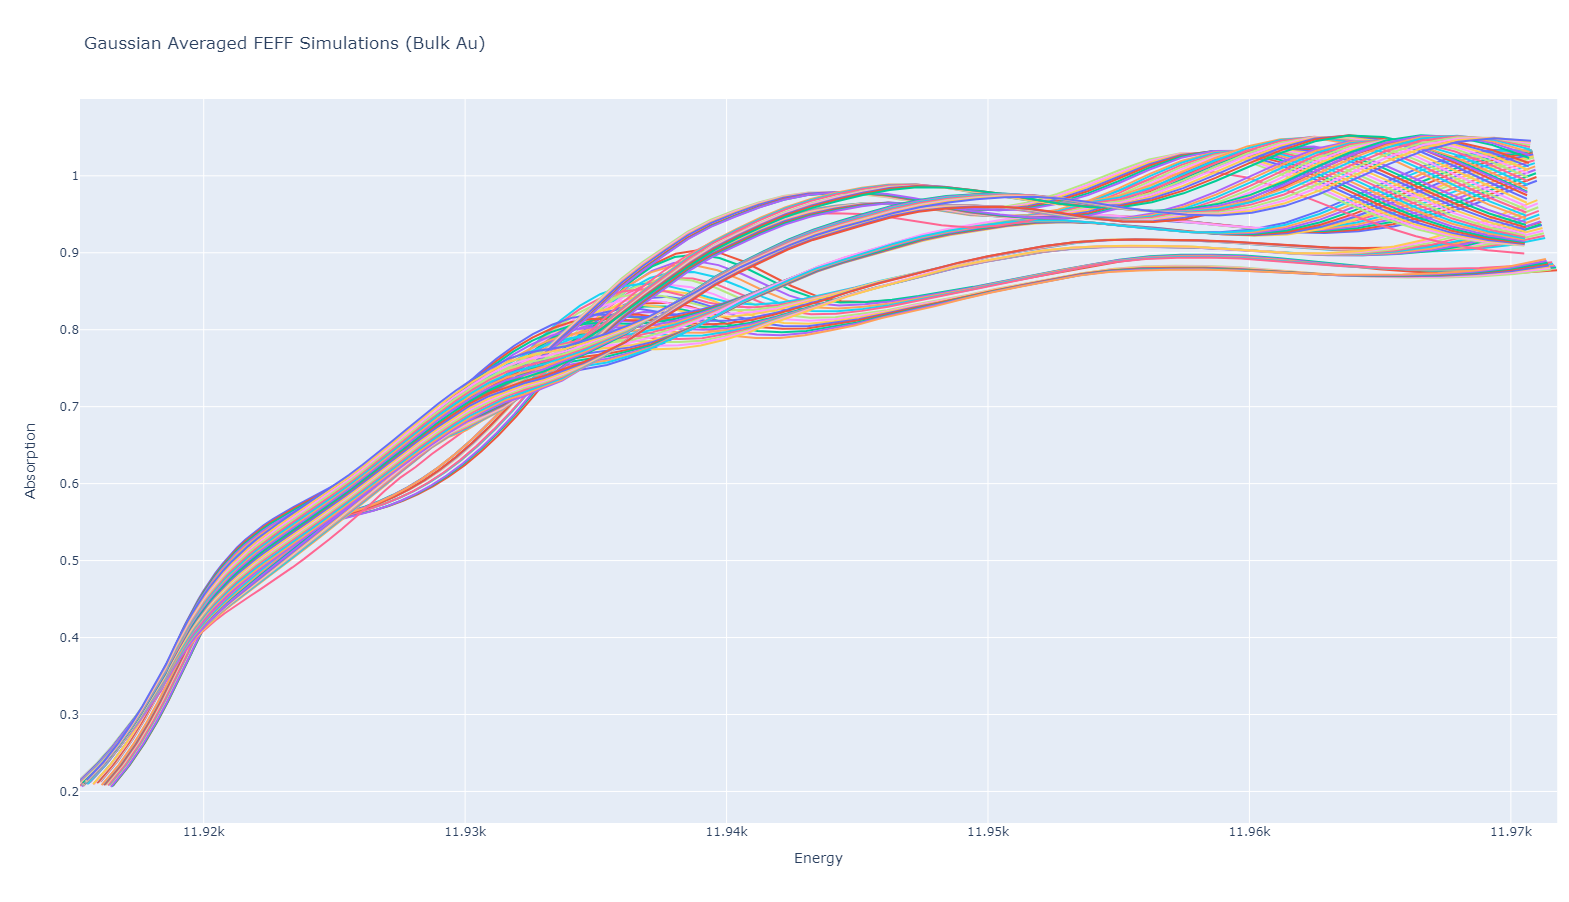
\includegraphics[width=\linewidth]{Chapters/Figures/newplot.png}
	\caption[FEFF Simulations Results]{Each spectrum represents the FEFF simulation results for a different distorted structure. For each spectrum, the crystal structure and center absorber remain constant, the only parameter that varies is the euclidean distance from the center to the other coordinates.}
	\label{fig:feff-results}
\end{figure}

\subsection{Generating Disorder via Probability Distribution Averaging}

One way to characterize system disorder is with the Gaussian standard deviation, $ \sigma $, of the radial distribution function. The idea of our statistical averaging method is to emulate this width by weighting the simulated XANES spectra according to this distribution. For example, Figure \ref{fig:gaussian-weighting-hist} depicts a histogram with $ \sigma=0.1 $~\AA. Each histogram bin represents a simulated XANES spectrum with a different isotropic displacement. For example, the bin at $ \Delta\rho=0.0 $~\AA~represents the simulated XANES spectrum with no distortion, and the bin at $ \Delta\rho=-0.2 $~\AA~represents the simulated XANES spectrum with all the atomic coordinates shifted isotropically inwards towards the center absorber by $ 0.2 $~\AA. The height of each bin, $ f(\Delta\rho) $, represents the relative contribution of each simulated XANES spectrum towards the resulting weighted spectrum. For visual clarity, Figure \ref{fig:gaussian-weighting-hist} depicts only 40 bins; the actual weighting includes 91 bins ranging from $ -0.45 $~\AA~to~$ +0.45 $~\AA.

% figure created in playground.ipynb
% !htb
\begin{figure}[h!]
	\centering
	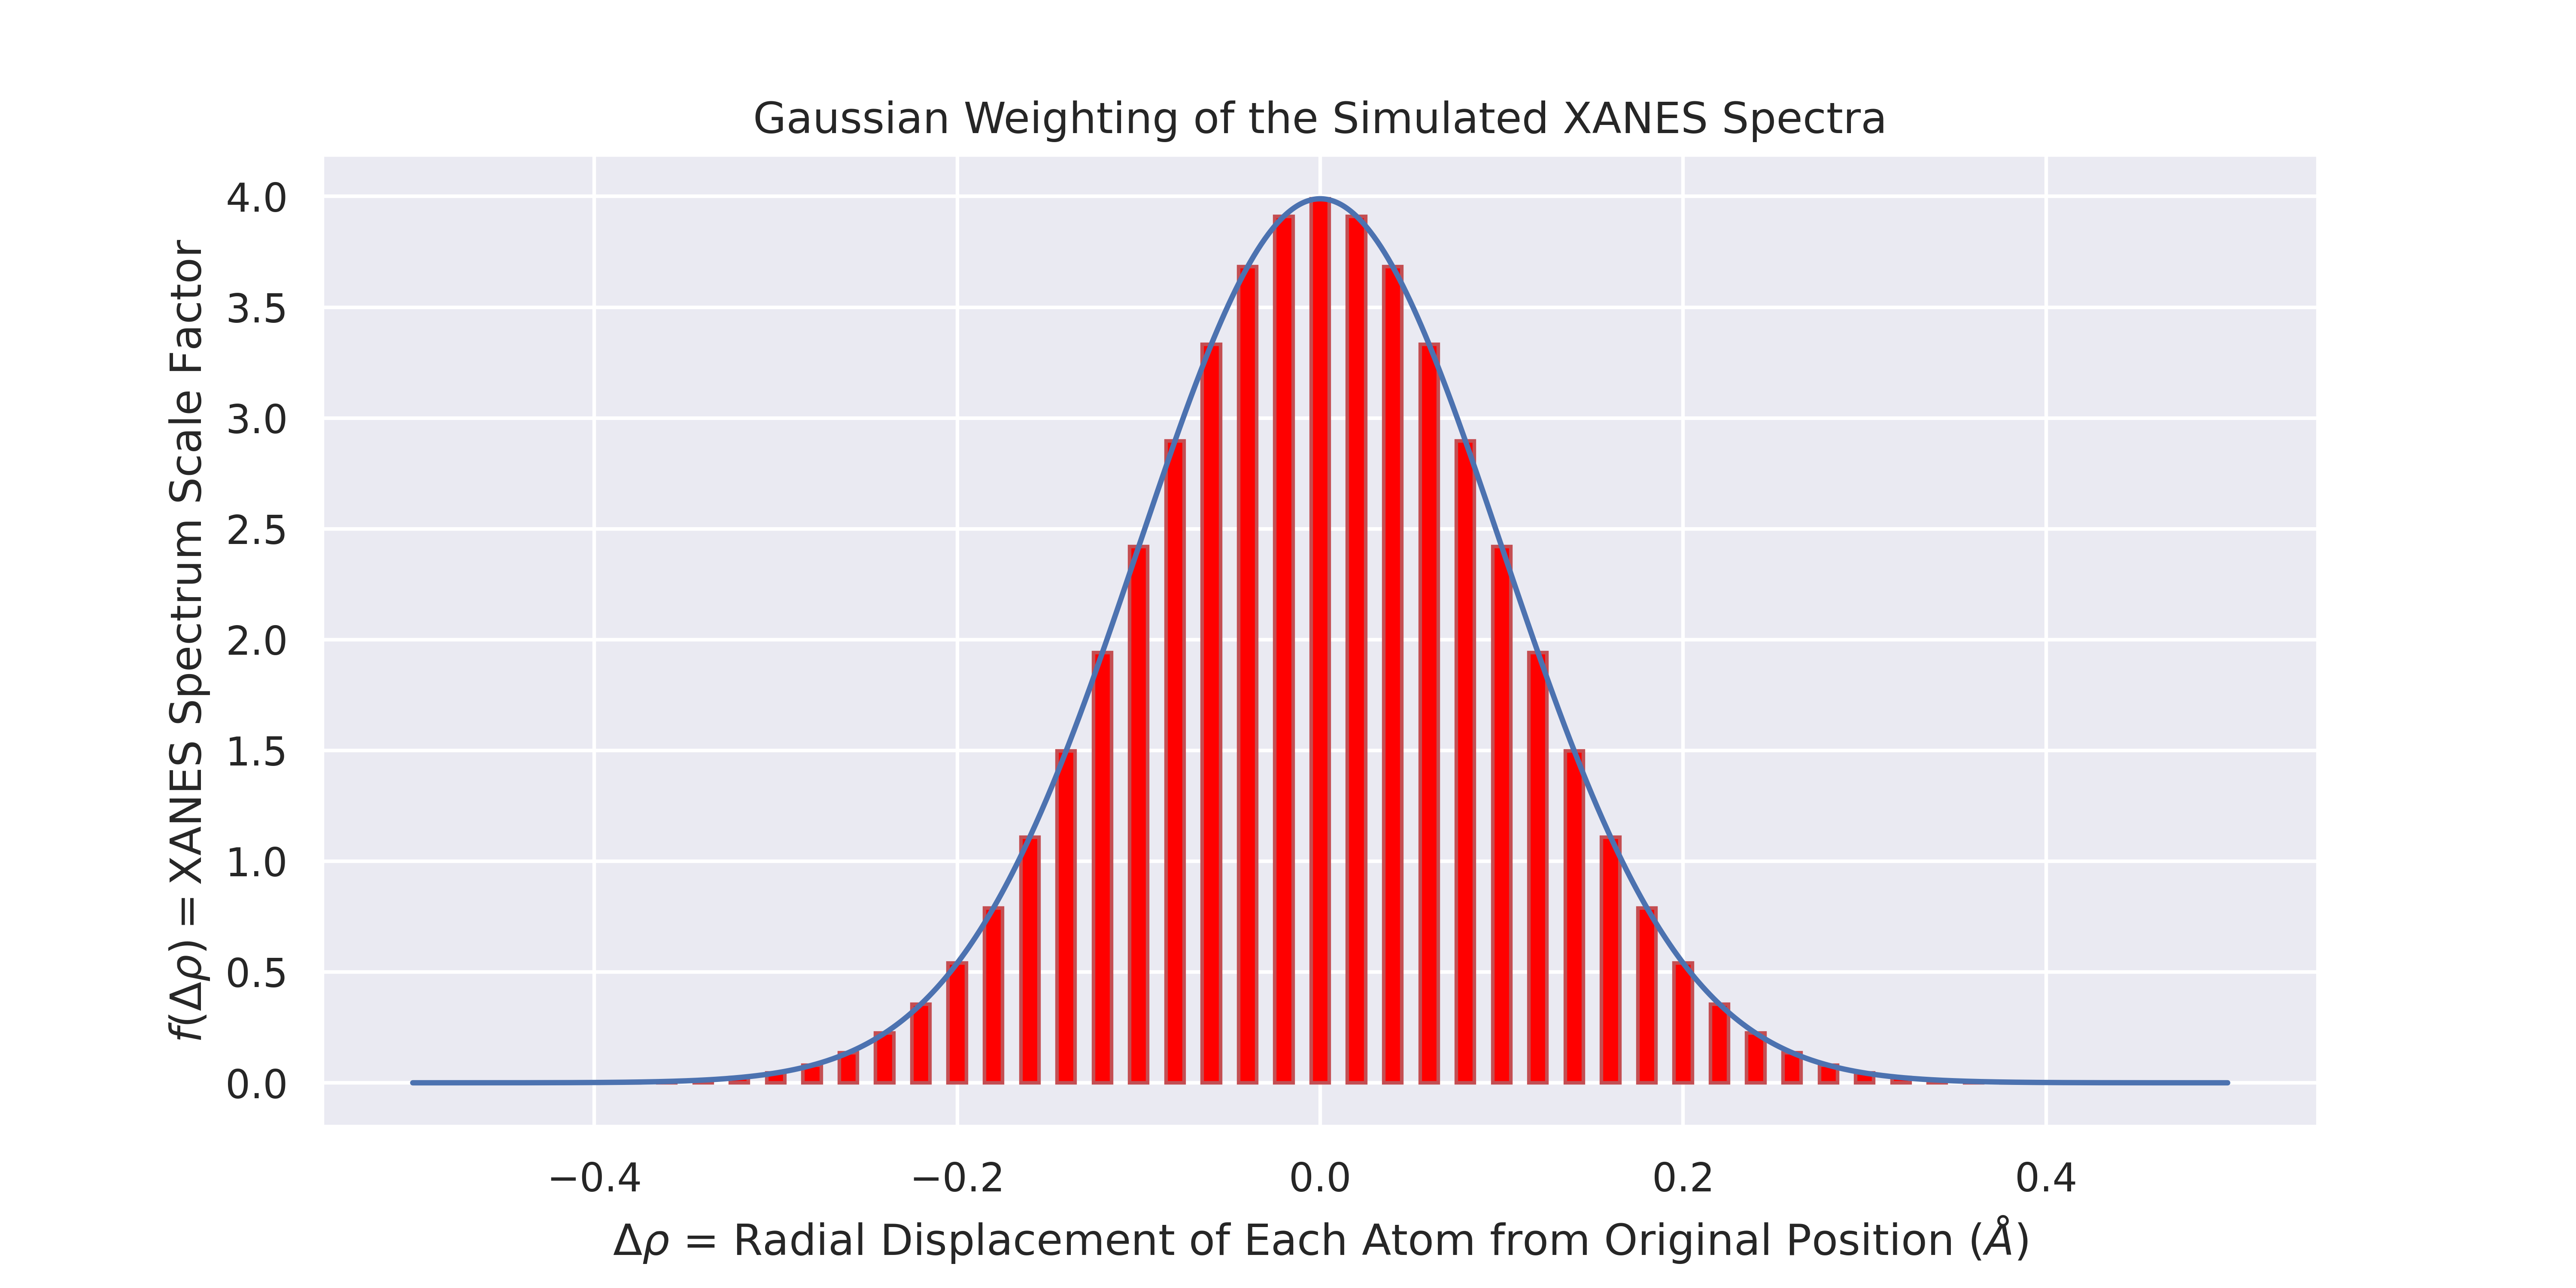
\includegraphics[width=\linewidth]{Chapters/Figures/gaussian-weighting-hist.png}
	\caption[Simulated Spectrum Gaussian Weighting]{A Gaussian distribution probability density function can be used to calculate the relative weight of each FEFF-generated XANES spectrum towards one simulated, disordered spectrum. Each bin (red bar) represents a FEFF-generated spectrum; the $x$-axis is the isotropic shift of the first nearest neightbor atomic positions, and the $y$-axis is the relative weight factor.}
	\label{fig:gaussian-weighting-hist}
\end{figure}

The disordered, Gaussian-averaged XANES spectrum, $ \left\langle \mu(E) \right\rangle $, using the histogram weighting of the gaussian in Figure \ref{fig:gaussian-weighting-hist} is calculate via Equation (\ref{eqn:gaussian-averaging}):

\begin{equation}
	\label{eqn:gaussian-averaging}
	\left\langle \mu(E) \right\rangle  = \frac{1}{S} \sum_{\Delta\rho=-.45}^{+.45} g\left(\Delta \rho \mid \mu=0, \sigma=0.1\right) \mu(E \mid \Delta\rho)
\end{equation}

\noindent
In the above equation, $ \Delta\rho $ is the isotropic radial displacement of each atom from its original position, $\mu(E \mid \Delta\rho) $ is the simulated FEFF spectrum for the given $ \Delta\rho $ configuration, and $ S $ represents a standardization factor included to negate the effect of the changing Gaussian height as a function of the variance, $ \sigma^2 $. With the inclusion of $ S $, only the relative height of each bin matters for producing the averaged XANES spectrum. This standardization factor is defined in Equation (\ref{eqn:gaussian-standardization}):

\begin{equation}
	\label{eqn:gaussian-standardization}
	S = \sum_{\Delta\rho=-.45}^{+.45} g\left(\Delta \rho \mid \mu=0, \sigma=0.01\right)
\end{equation}

\noindent
In both equations (\ref{eqn:gaussian-averaging}) and (\ref{eqn:gaussian-standardization}), the function $ g $ is just the typical Gaussian distribution probability density function (Equation \ref{eqn:gaussian}): 

\begin{equation}
	\label{eqn:gaussian}
	g(x) = \frac{1}{{\sigma \sqrt {2\pi } }}e^{{{ - \left( {x - \mu } \right)^2 } \mathord{\left/ {\vphantom {{ - \left( {x - \mu } \right)^2 } {2\sigma ^2 }}} \right. \kern-\nulldelimiterspace} {2\sigma ^2 }}}
\end{equation}

The above example only generates one (simulated) disordered XANES spectrum and does so via weighting of a Gaussian distribution with mean and variance equal to $ 0 $ and $ 0.01 $, respectively. To simulate systems with different degrees of disorder, we can vary the shape of the probability density function. With a Gaussian distribution, we can only vary the mean and variance; to simulate even more conditions, however, we can instead use the multivariate skew-normal distribution, $ f(x) $ \cite{skewnorm_Azzalini_1999} \cite{2020SciPy-NMeth}, written in equation (\ref{eqn:skew-norm}). 

\begin{equation}
	\label{eqn:skew-norm}
	f(x)=2\phi (x)\Phi (\alpha x)
\end{equation}
 
\noindent
where $ \phi(x) $ is the Gaussian PDF:
\begin{equation}
	\label{eqn:skew-norm-pdf}
	\phi (x)={\frac  {1}{{\sqrt  {2\pi }}}}e^{{-{\frac  {x^{2}}{2}}}}
\end{equation}

\noindent
and $ \Phi (x) $ is the Gaussian CDF:
\begin{equation}
	\label{eqn:skew-norm-cdf}
	\Phi (x)=\int _{{-\infty }}^{{x}}\phi (t)\ dt
\end{equation}

%------------WIKIPEDIA EQUATION VERSION -------------
% \begin{equation}
% 	\label{eqn:skew-norm-cdf}
% 	\Phi (x)=\int _{{-\infty }}^{{x}}\phi (t)\ dt={\frac  {1}{2}}\left[1+\operatorname {erf}\left({\frac  {x}{{\sqrt  {2}}}}\right)\right]
% \end{equation}
% \noindent
% and erf is Gauss' error-function

% \begin{equation}
% 	\label{eqn:skew-norm-cdf-erf}
% 	{\displaystyle \operatorname {erf} \left(z\right)={\frac {2}{\sqrt {\pi }}}\int _{0}^{z}e^{-t^{2}}\,dt}
% \end{equation}

\noindent
Equation (\ref{eqn:skew-norm}) includes the shape parameter, $ \alpha $, which has the nice property of producing a right-skewed distribution when positive and a left-skewed distribution when negative. When $ \alpha=0 $, the distribution simply produces the typical Gaussian distribution (\ref{eqn:gaussian}). Utilizing equation (\ref{eqn:skew-norm}), we can vary $ \mu, \sigma,  $ and $ \alpha $ to alter the first four moments of the function: the mean, standard deviation, skew, and kurtosis. Eighteen possible skew-norm weighting functions are plotted in Figure \ref{fig:skew-norm-options}, however, 1000+ unique combinations of weightings would be required to produce the neural network's training data.

\begin{figure}[h!]
	\centering
	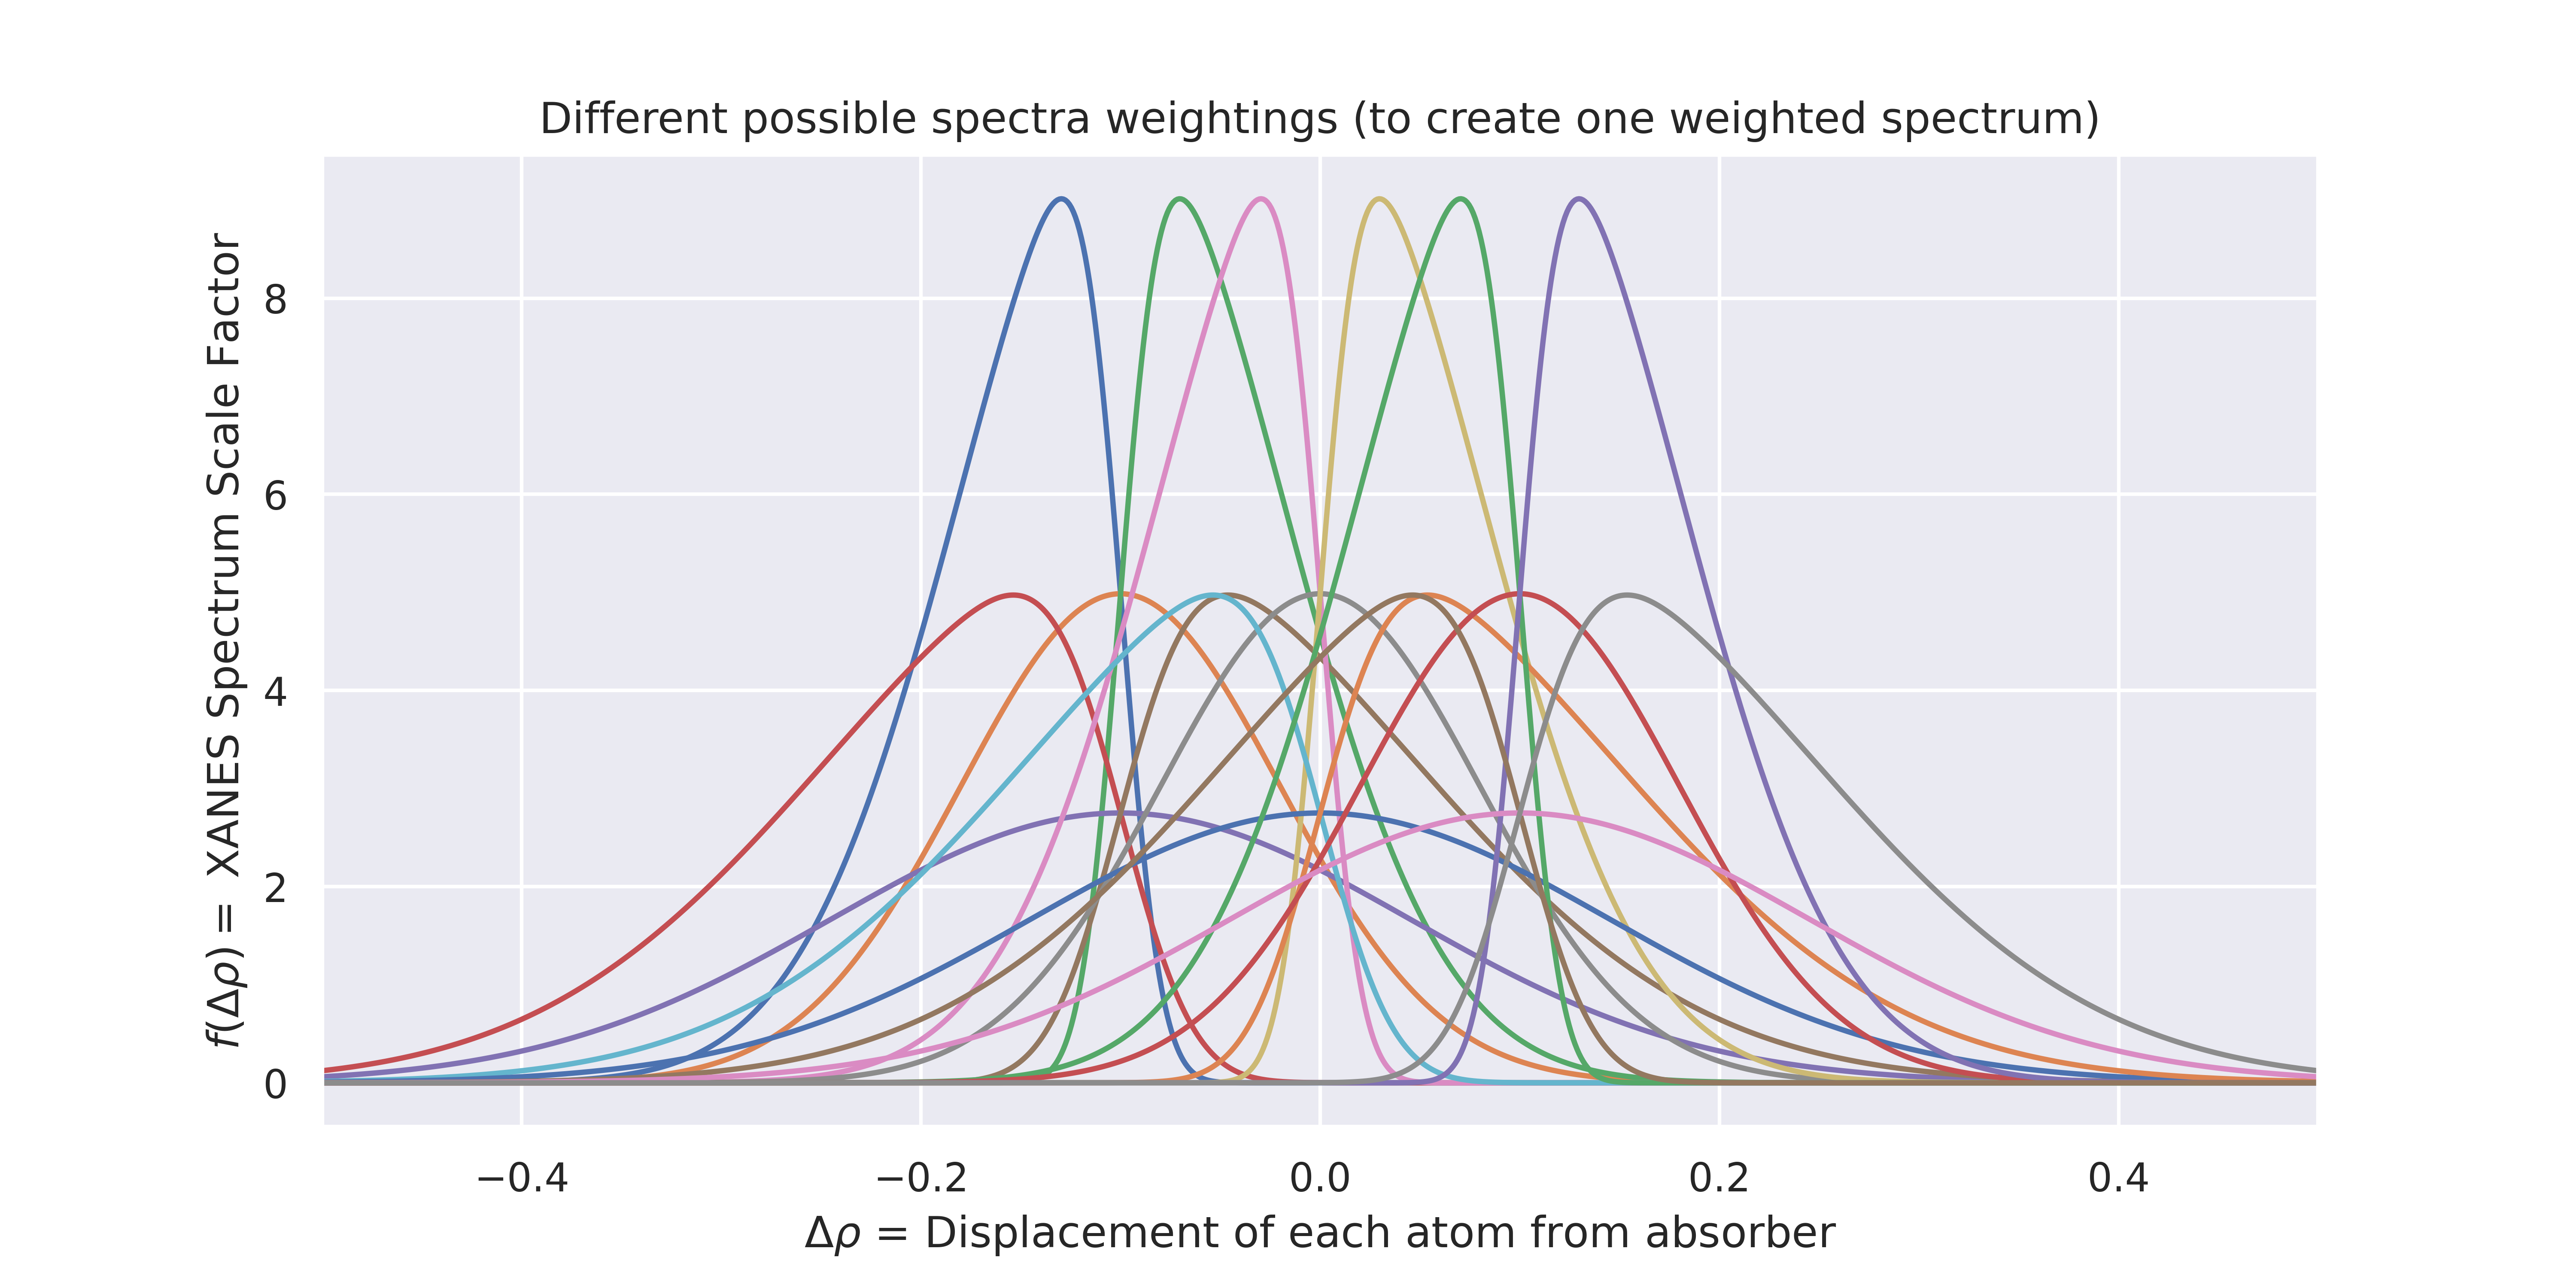
\includegraphics[width=\linewidth]{Chapters/Figures/skewnorm_options.png}
	\caption[Simulated Disordered Spectrum Weightings]{Eighteen skew-norm distributions plotted with all possible combinations of ${\sigma \in \{.08, .145\} }$, $ \mu \in \{-.1, 0, .1\} $, and $ \alpha \in \{-5,0,5\} $. Each represents a possible way to produce a simulated, disordered spectrum from many FEFF-simulated, distorted spectra} 
	\label{fig:skew-norm-options}
\end{figure}

The disorder of the skew-norm-generated, disordered spectrum is characterized by the mean squared displacement of each atom from its original position ($ \Delta\rho $ ), weighted in the same manner as the spectra. Note, this is different than the standard deviation of the Gaussian used to create it. The weighted mean squared displacement, $ MSD $, is calculated via as follows:

% original weighting, no longer used
% \begin{equation}
% 	\label{eqn:weighted-MSD}
% 	MSD  = \frac{1}{S} \sum_{\Delta\rho=-.45}^{+.45} f\left(\Delta \rho \mid \mu, \sigma^2, \alpha \right) 
% \end{equation}
% and the $ MSD $  of each individual FEFF spectrum is equal to the isotropic distortion, $ \Delta\rho $. 

\begin{align}
	\label{eqn:updated-weighted-MSD}
	S &= \sum_{\Delta\rho=-.45}^{+.45} f\left(\Delta \rho \mid \mu, \sigma^2, \alpha \right) \\
	\mu_{weighted} &= \frac{1}{S} \sum_{\Delta\rho=-.45}^{+.45} \Delta\rho \left( f ( \Delta \rho \mid \mu, \sigma^2, \alpha ) \right) \\
	MSD &= \frac{1}{S} \sum_{\Delta\rho=-.45}^{+.45} \Delta \rho \left( f ( \Delta \rho \mid \mu, \sigma^2, \alpha ) - \mu_{weighted} \right) ^2
\end{align}

\noindent Here, $ f $ is the skew-norm function from equation (\ref{eqn:skew-norm}). The code for this equation can be found in Appendix \ref{appendix:gaussianator}, written in Python and optimized with NumPy \cite{numpy}.

\subsection{Simulation vs. Experimental Data} \label{sec:end-disorder}

To check our FEFF simulation parameters, as well as the validity of the Gaussian-weighted disorder technique, we compare the simulation data to experimental data \cite{au-nanowires-silca-wang} \cite{crooks-55nm-au-exp} \cite{jing-au-nanoparticle-exp} \cite{au-nanowires-silca-wang}. In Figure \ref{fig:avg-experimental-vs-simulation}, both experimental and simulation spectra for bulk-like and nanoparticle scenarios are plotted. EXAFS fitting was used to characterize the disorder in the experimental measurements. For the bulk foil, this parameter was found to be $ \sigma^2=0.0081(5)~{\AA}^2 $, and for the 8~nm disordered particle, $ \sigma^2=0.0102(8) $~{\AA}$ ^2 $.  One simulated disordered spectrum was weighted according to the Gaussian $ N(0, 0.09) $ to represent the disordered nanoparticle, and the other was weighted according to the gaussian $ N(0, 0.038)  $ to represent the bulk. These weightings correspond to $ MSD $ values that match the measured $ \sigma^2 $ values for the experimental data.  

\begin{figure}[h]
	\centering
	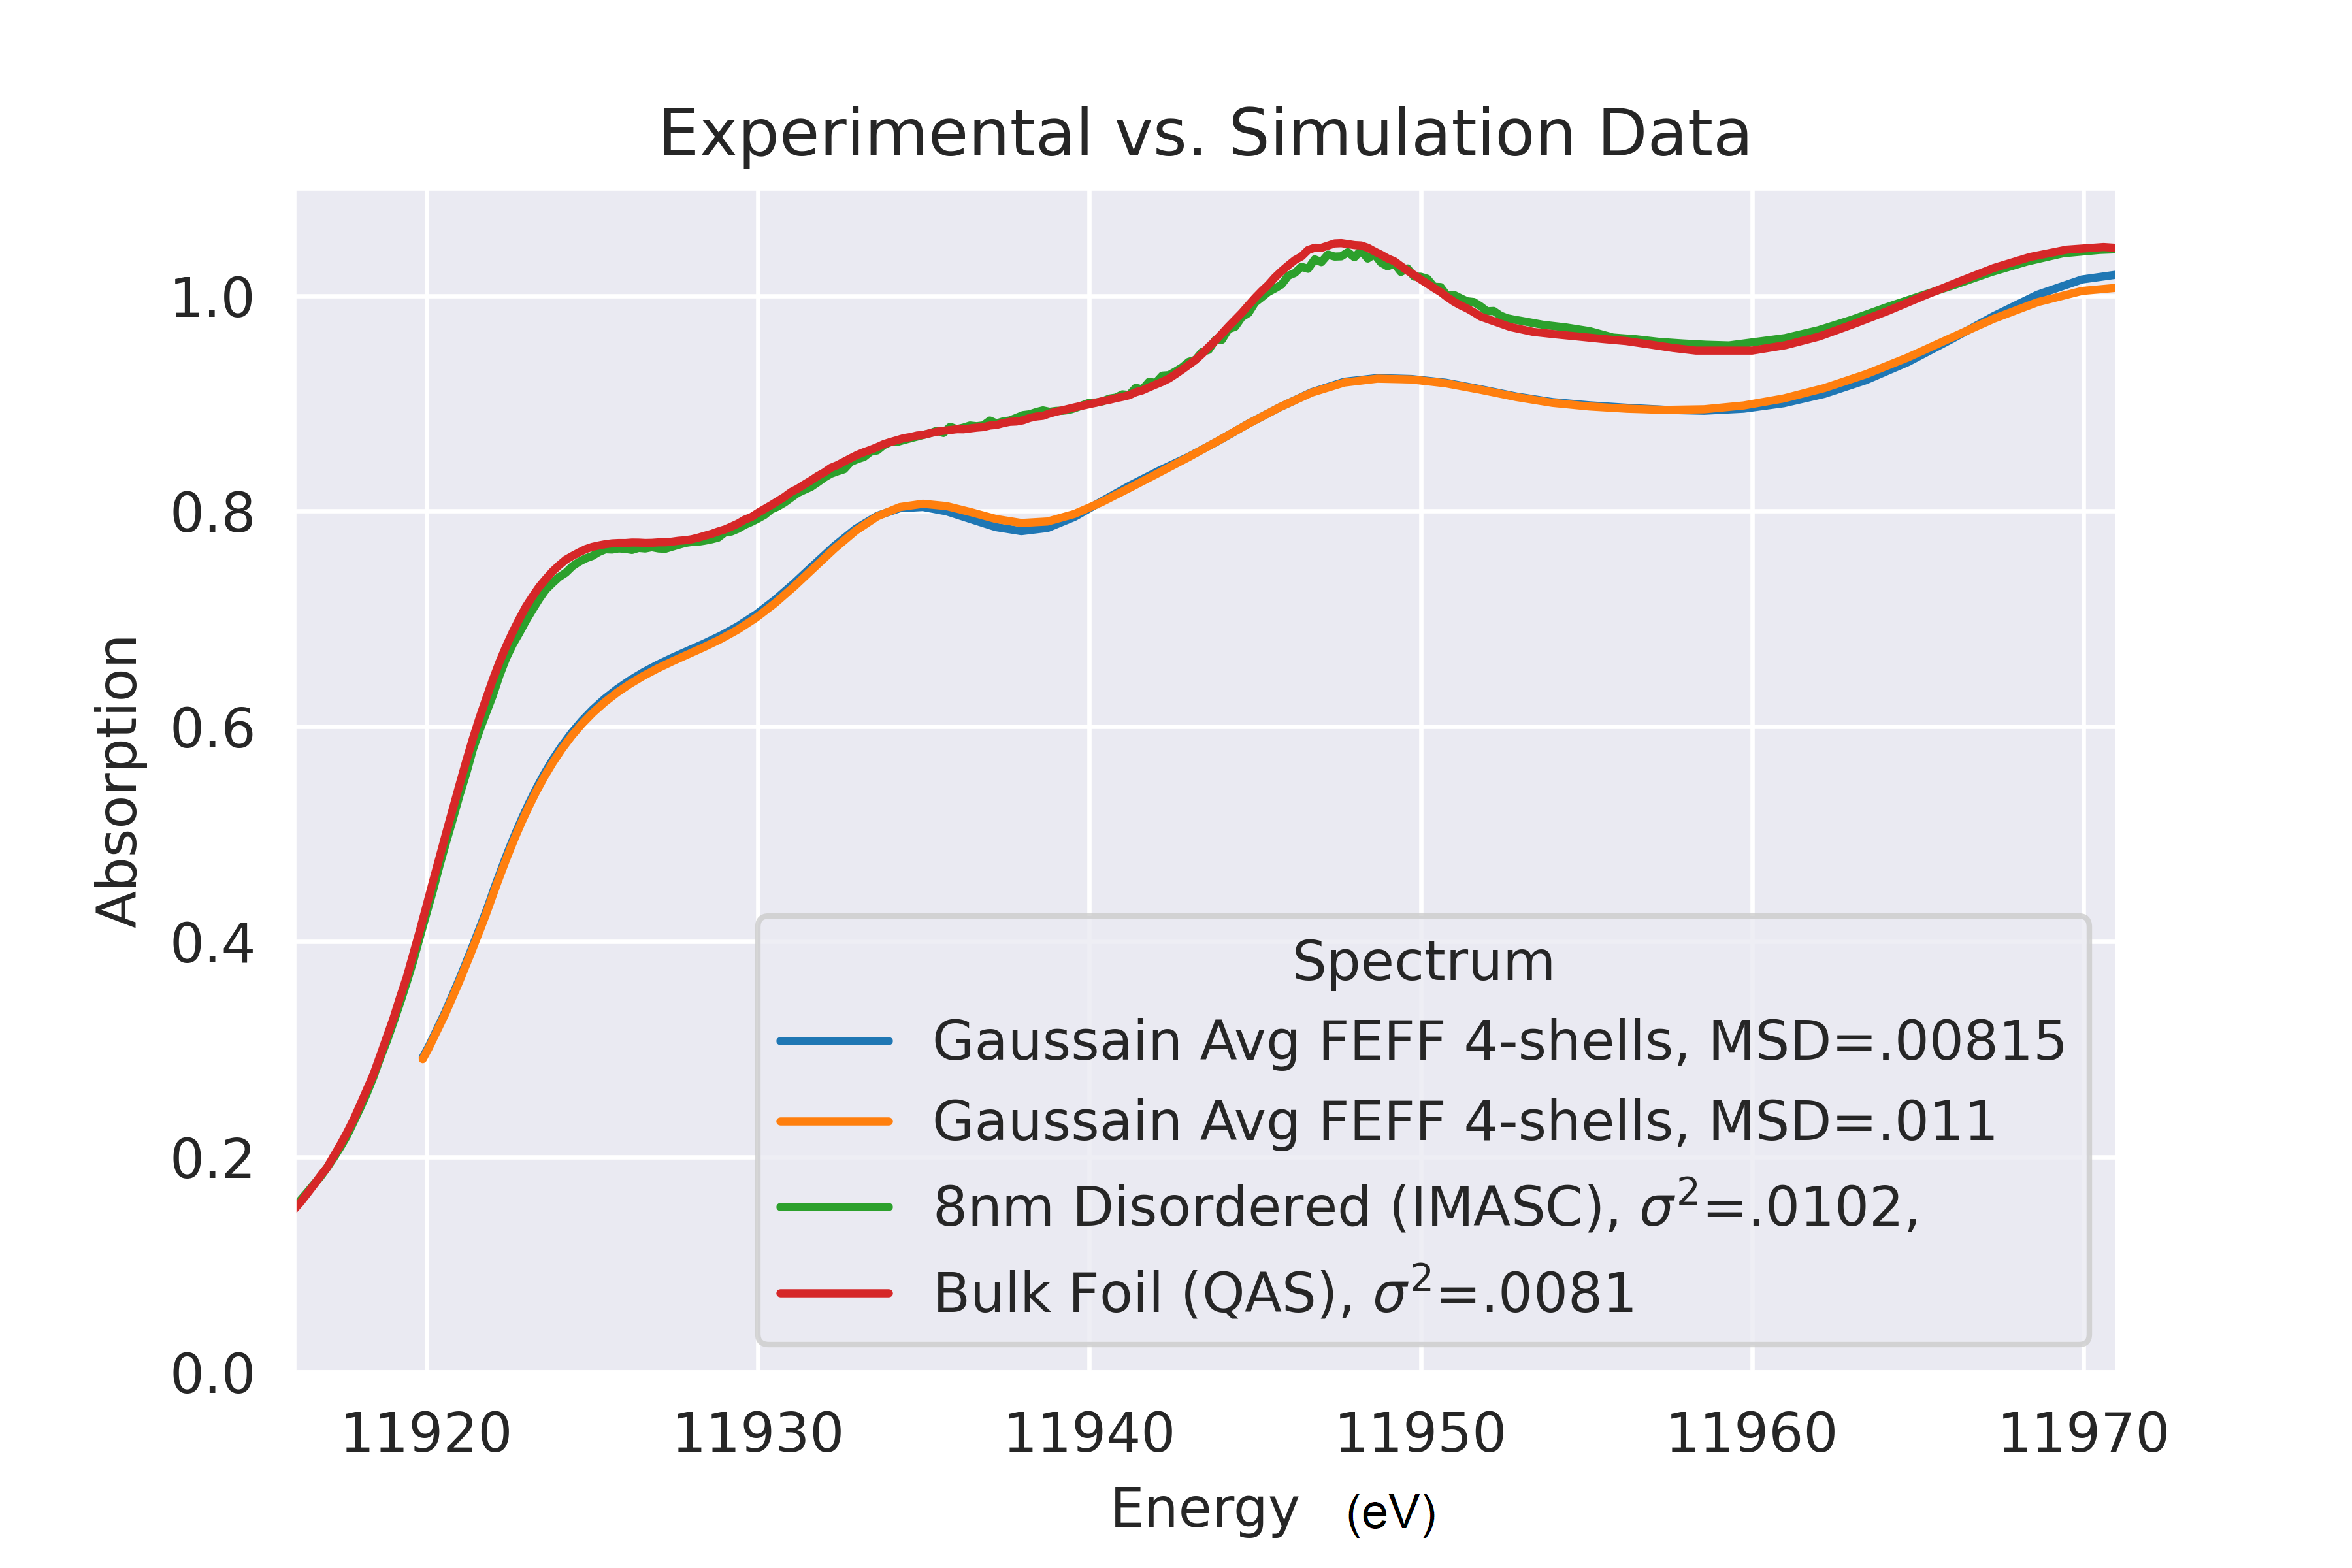
\includegraphics[width=.75\linewidth]{Chapters/Figures/updated_bulk_8nm_disorder_experimental_theory_comparison.png}
	\caption[Simulation vs. Experimental]{Comparing the bulk foil (red) measurement to the 8~nm disordered nanoparticle (green) measurement is an analog to comparing the simulated, non disordered FEFF spectrum (blue) to the simulated disordered spectrum (orange).}
	\label{fig:avg-experimental-vs-simulation}
\end{figure}

In Figure \ref{fig:avg-experimental-vs-simulation}, the bulk Au foil spectrum is above the 8~nm nanoparticle spectrum (more absorption) until the peak around 11937~eV, where the nanoparticle's absorption becomes higher. The two criss-cross again over the next two peaks, changing which material has the higher absorbance in an energy range. This change is more easily seen in Figure \ref{fig:avg-experimential-vs-simulation-difference}, which plots the difference between the bulk material and the nanoparticle absorption for both the experimental measurements and the simulations. The experimental and simulation difference-spectra follow the same trend with the exception of the peak around 11947~eV.
% The two spectrum switch again at the peak around 11943~eV so the bulk foil's absorption nlevel is higher again. Beyond this peak, the two


\begin{figure}[h!]
	\centering
	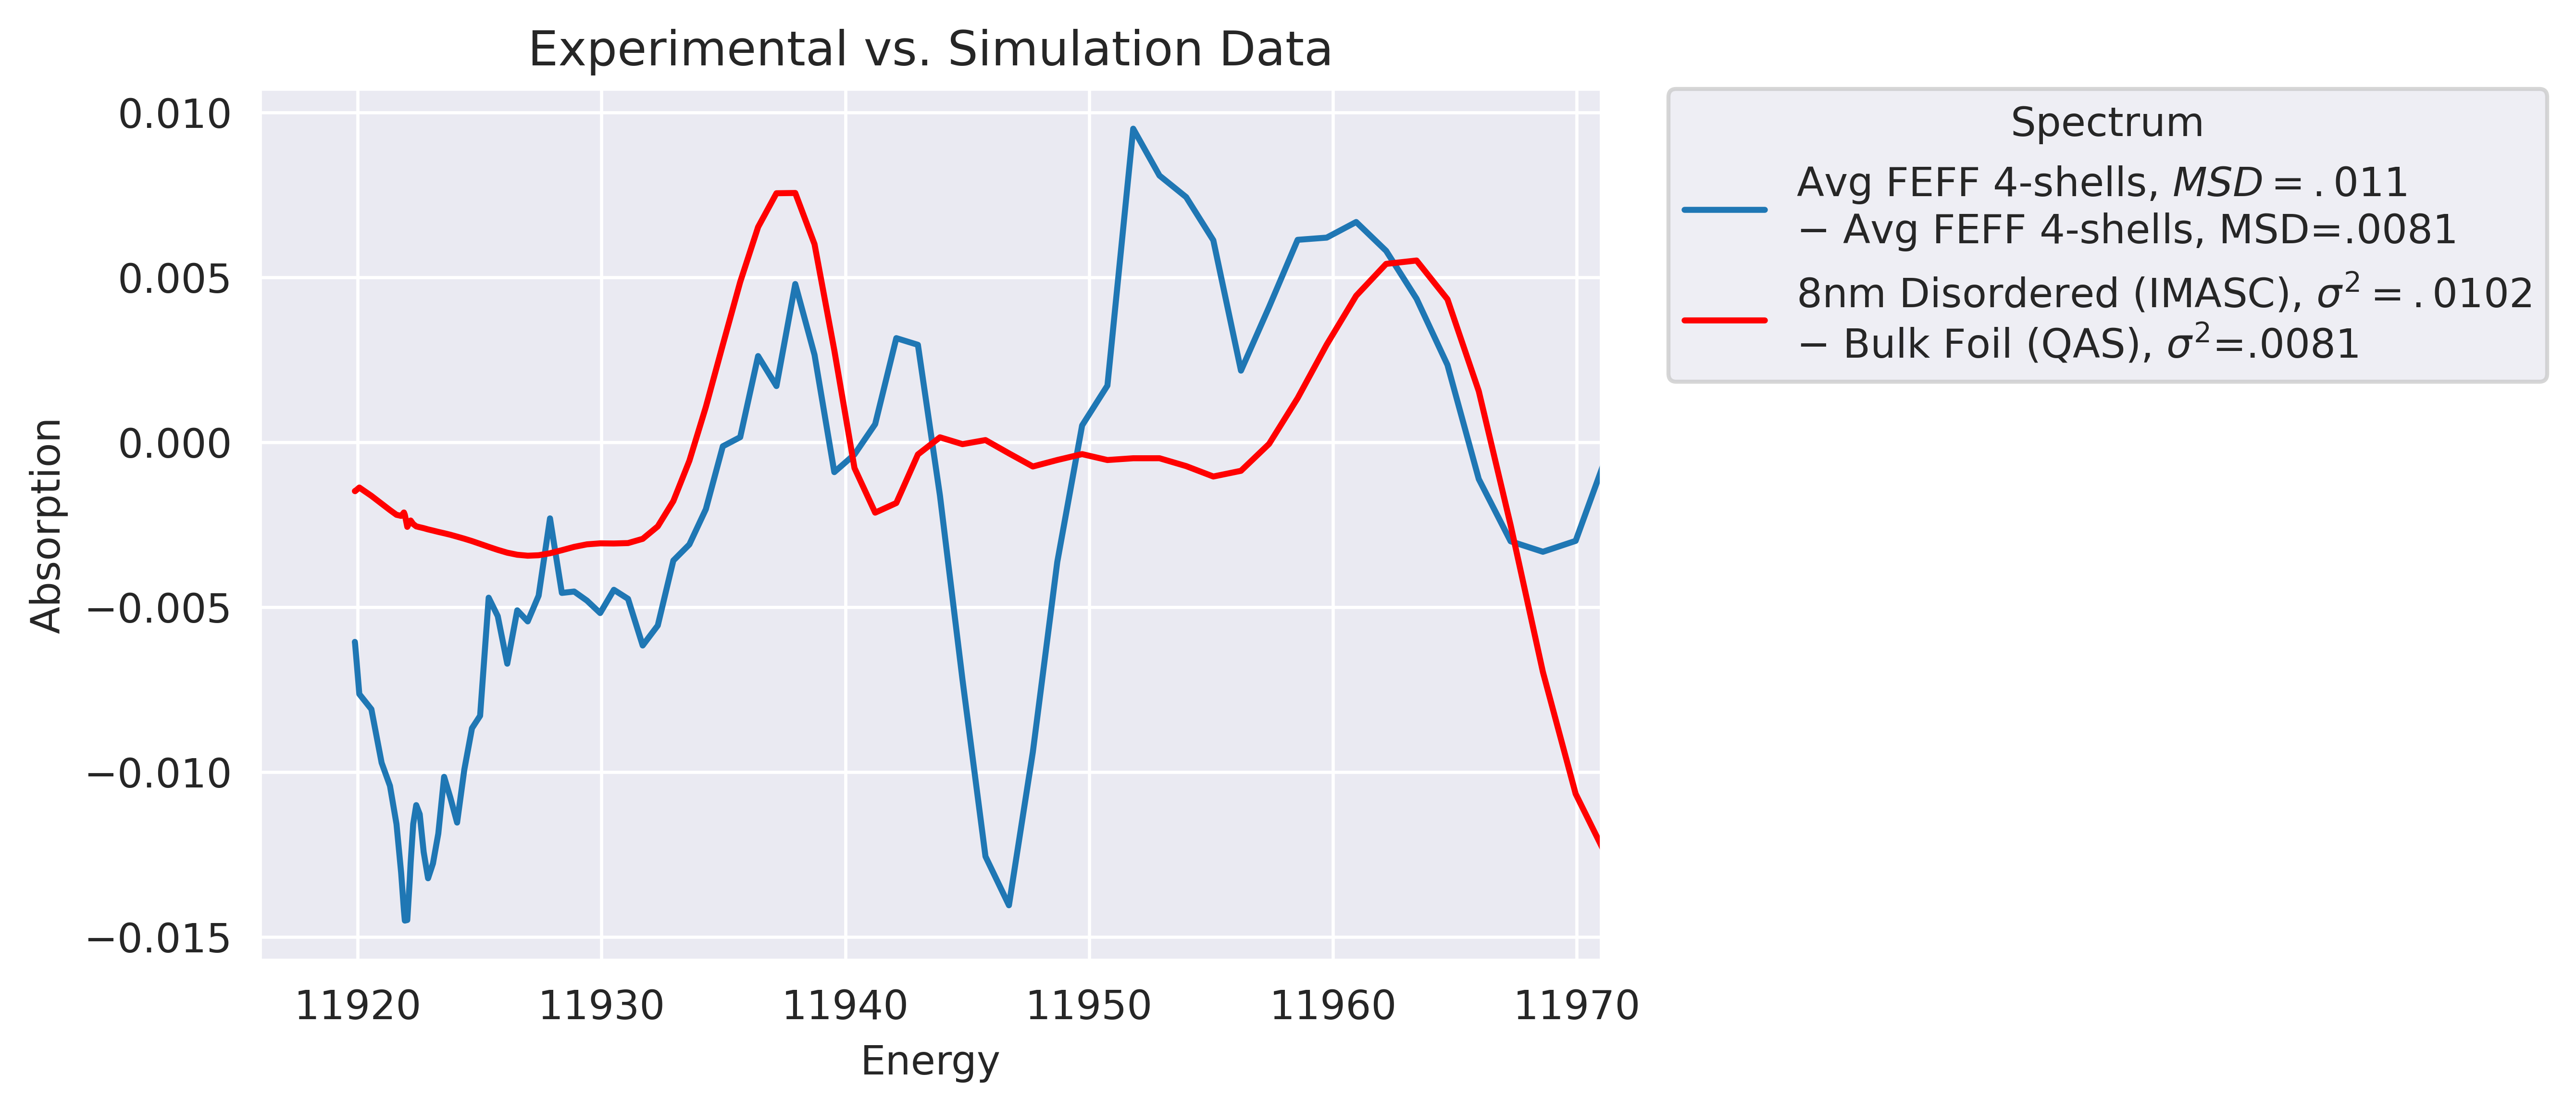
\includegraphics[width=\linewidth]{Chapters/Figures/experimental_vs_simulation_delta.png}
	\caption[Bulk-nanoparticle difference: Simulation vs. Experimental data]{The difference between the nanoparticle spectrum and the bulk spectrum are plotted for the same data as in Figure \ref{fig:avg-experimental-vs-simulation}. It is easier to see where the bulk and the nanoparticle absorption crisscross by plotting the difference.}
	\label{fig:avg-experimential-vs-simulation-difference}
\end{figure}

Figures \ref{fig:avg-experimental-vs-simulation} and \ref{fig:avg-experimential-vs-simulation-difference} are not meant to be perfect comparisons of simulations vs. experimental data. For one, the experimental data includes a comparison between a bulk spectrum to a nanoparticle. By contrast, both the simulation spectra are of the same size 55 atom cluster. Still, much of the disorder trends are coded in the simulation approach. 

To test if the size information is also coded in our simulations, we compare different size nanoparticle simulations to experimental data in Figure \ref{fig:avg-experimental-vs-simulation2}. We first simulated two different size nanoparticle gold clusters, one with 13 Au atoms and one with 55. As expected, including more atoms in the simulation produces more bulk-like spectrum characteristics, such as larger amplitude peaks.

\begin{figure}[h]
	\centering
	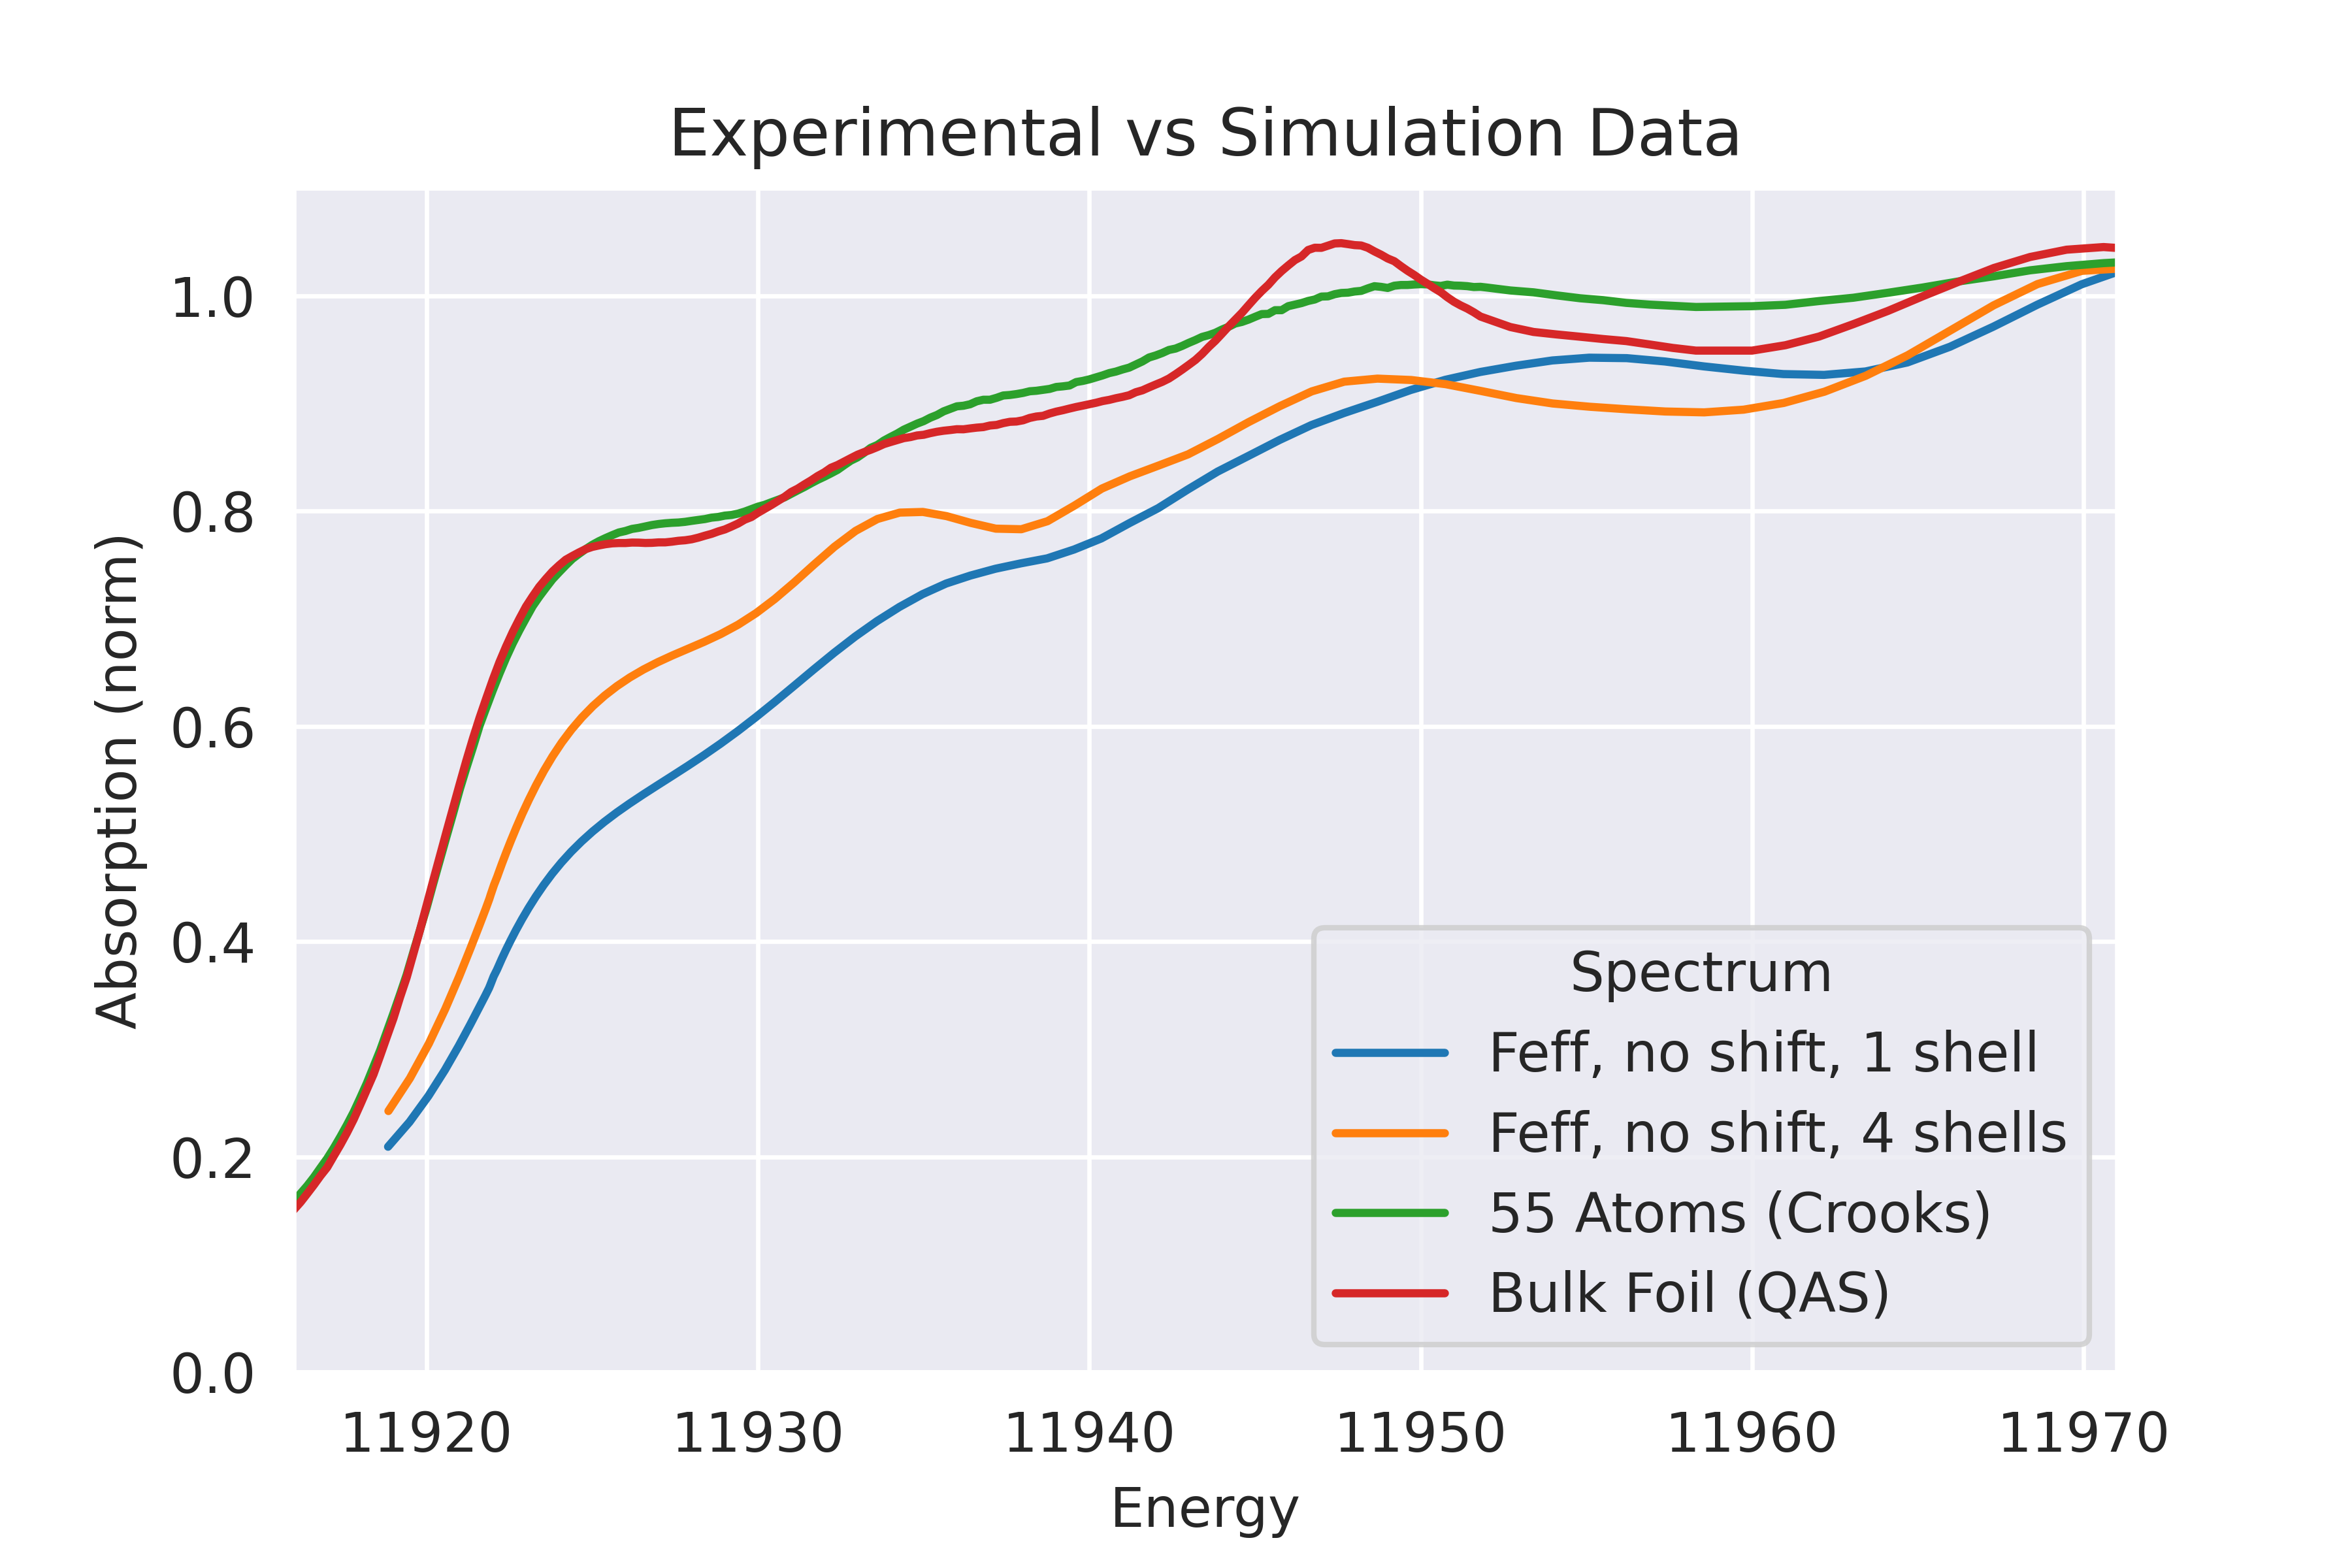
\includegraphics[width=.7\linewidth]{Chapters/Figures/Bulk_55atom_experimental_theory_comparison.png}
	\caption[Simulation vs. Experimental 2]{Comparing the bulk foil (red) measurement to the 55 atom nanoparticle (green) measurement is an analog to comparing the 13 atom simulated spectrum (blue) to the 55 atom simulated spectrum (orange).}
	\label{fig:avg-experimental-vs-simulation2}
\end{figure}


These preliminary indications suggest the statistical approach may provide useful insights given the similarity in trends; however, this does not yet provide any indication as to whether the statistical averaged simulations are equivilent to the particle average simulations, nor do they tell us whether these spectra would work for predicting the mean squared disorder from experimental spectra. This broader discussion is the topic of the next section.


\section{Particle-Averaged FEFF vs. Skewnorm-Averaged Structures} \label{sec:pa-feff-vs-gaussian-feff}

While it is important to see that the skew-norm-averaging methodology maintains the systematic changes in XANES spectra as disorder increases (as seen in section \ref{sec:end-disorder}), it is more important to compare this methodology to the widely-used particle-averaged methodology (seen in section \ref{sec:traditional-disorder})


% In the skew-norm methodology, we only calculate a center absorber because of symmetry. For simulating disordered structures, however, it is necessary to calculate all the absorbers. 


\begin{figure}[!h]
	\centering
	\label{fig:pa-vs-sknm-feff}
	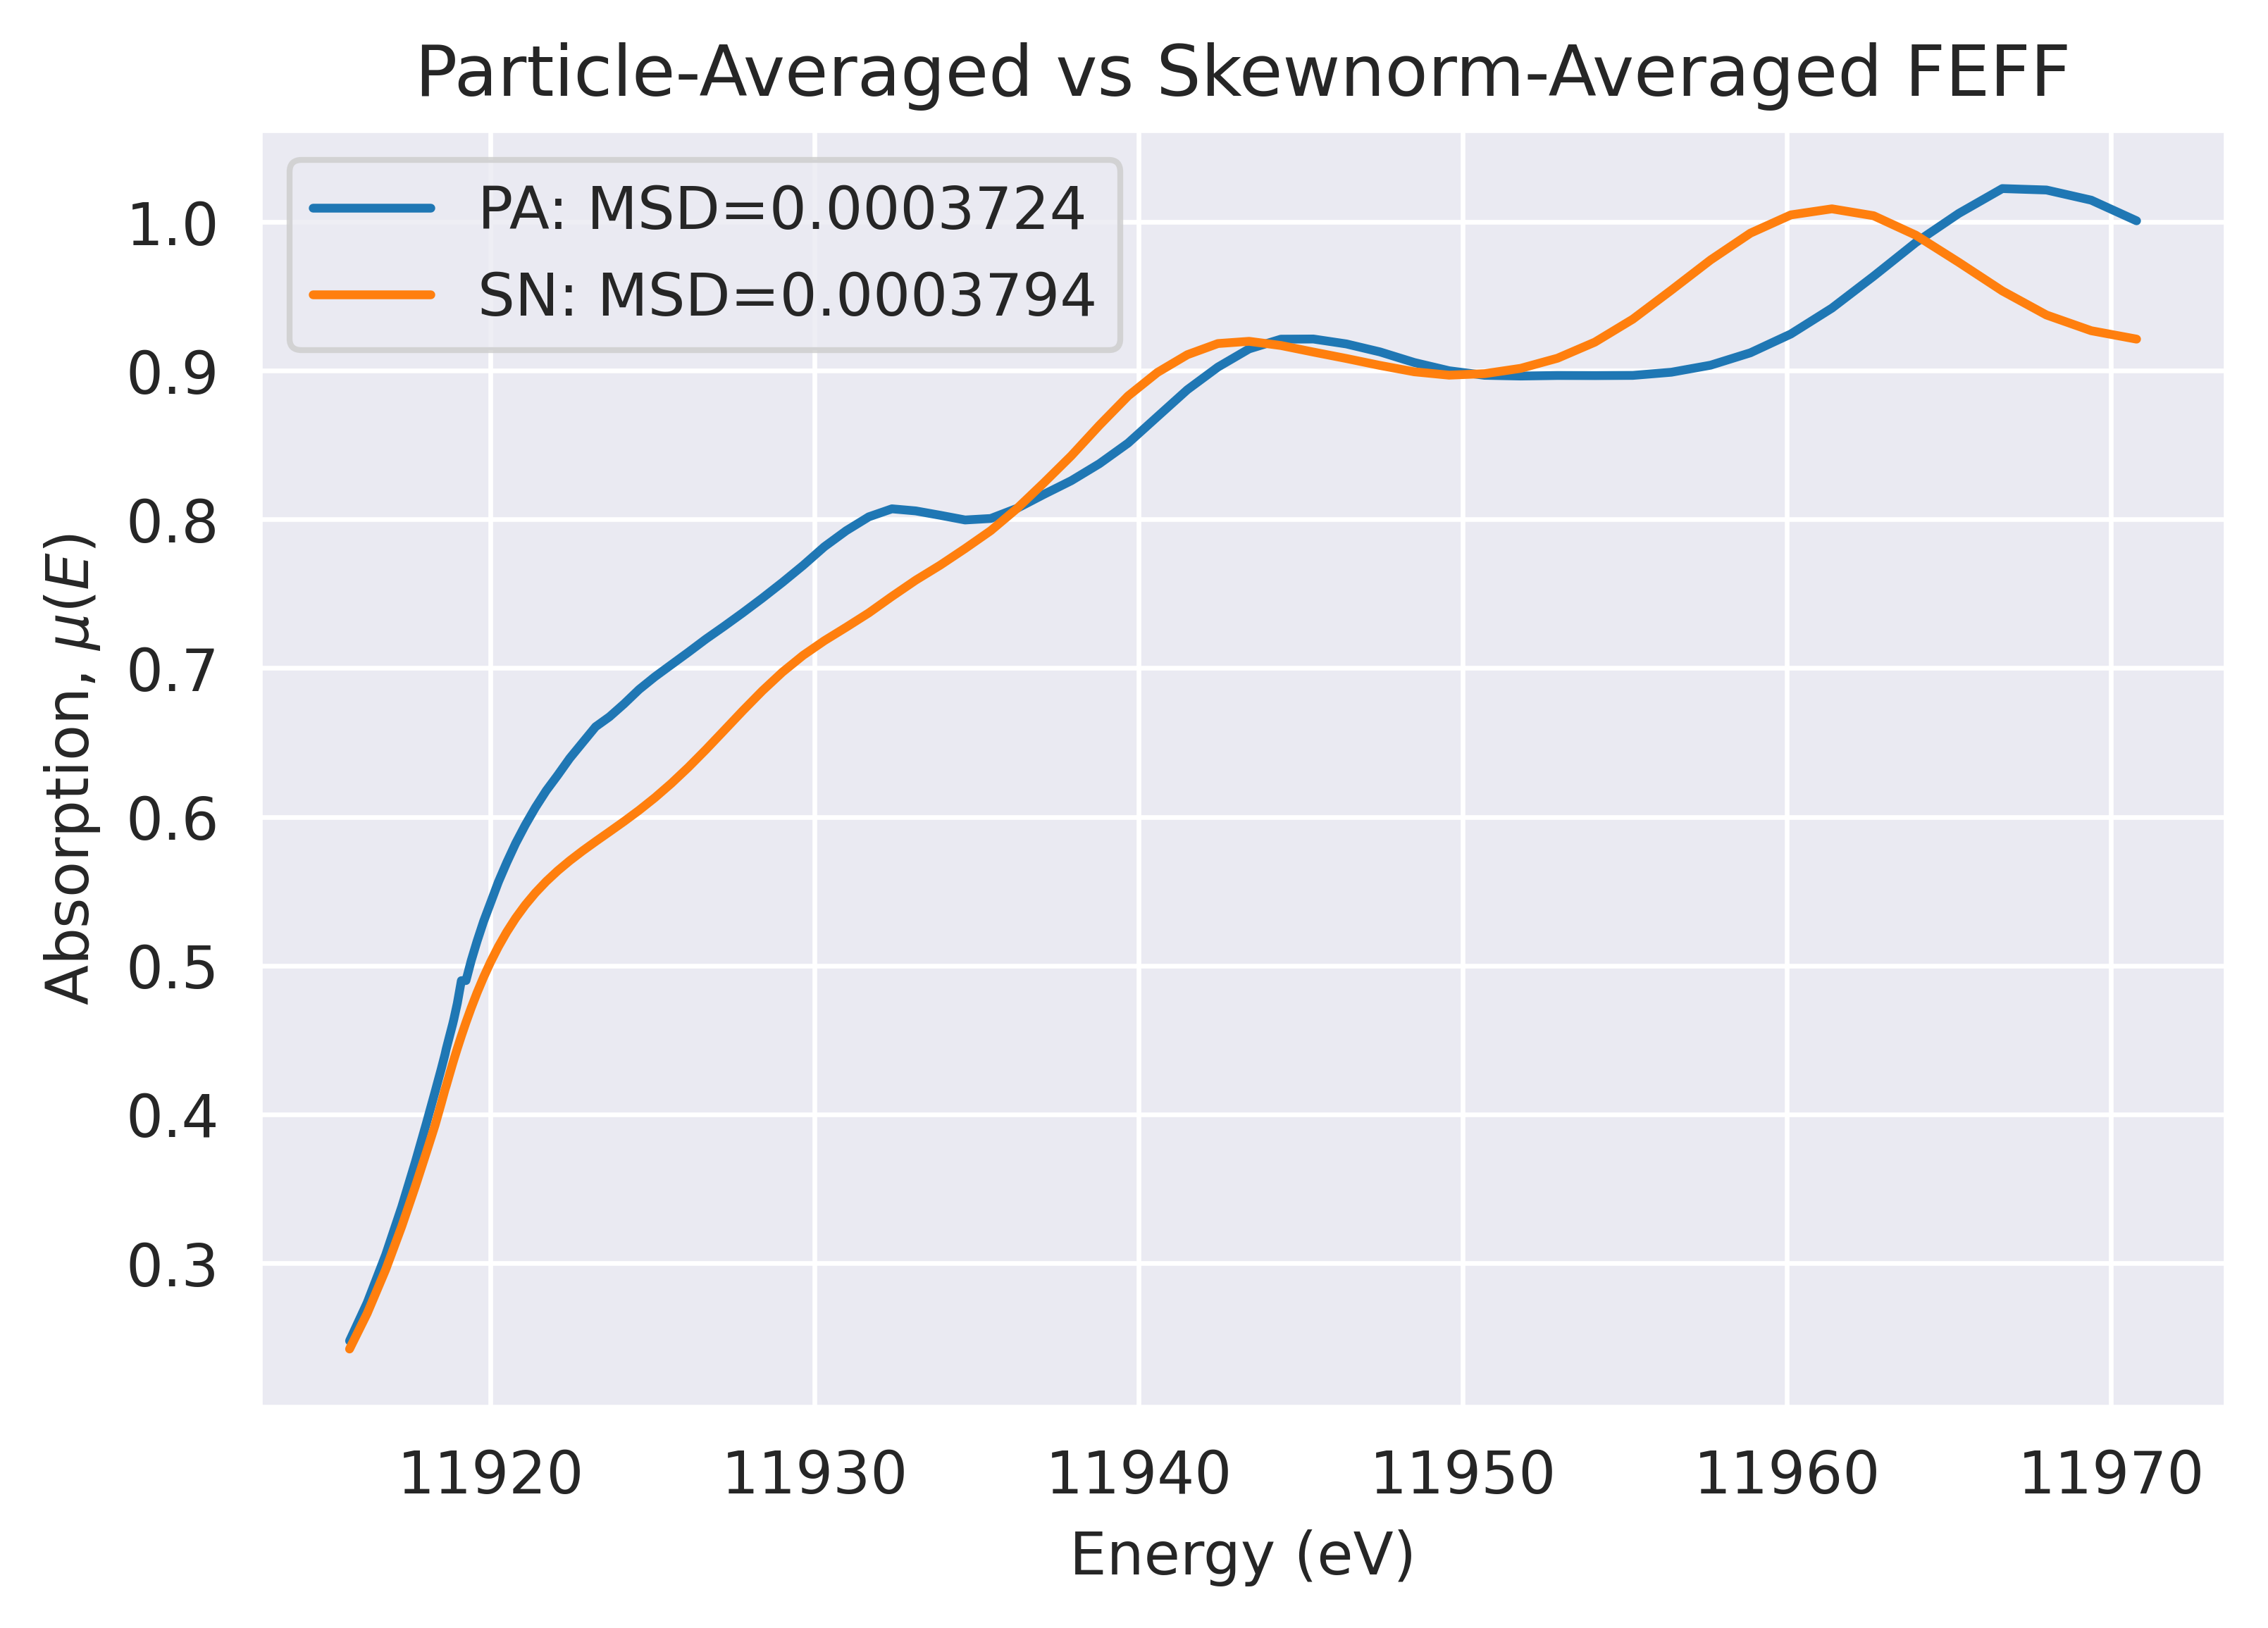
\includegraphics[width=.75\linewidth]{Chapters/Figures/PA-vs-skewnorm-newvals.png}
	\caption[Particle-Averaged vs. Skewnorm-Averaged FEFF Low-Disorder]{The particle Averaged FEFF vs. Skewnorm Averaged FEFF. The systematic difference reveal a flawed assumption in the skewnorm-Averaged Methodology}
\end{figure}

\begin{figure}[!h]
	\centering
	\label{fig:pa-vs-sknm-feff-bigmsd}
	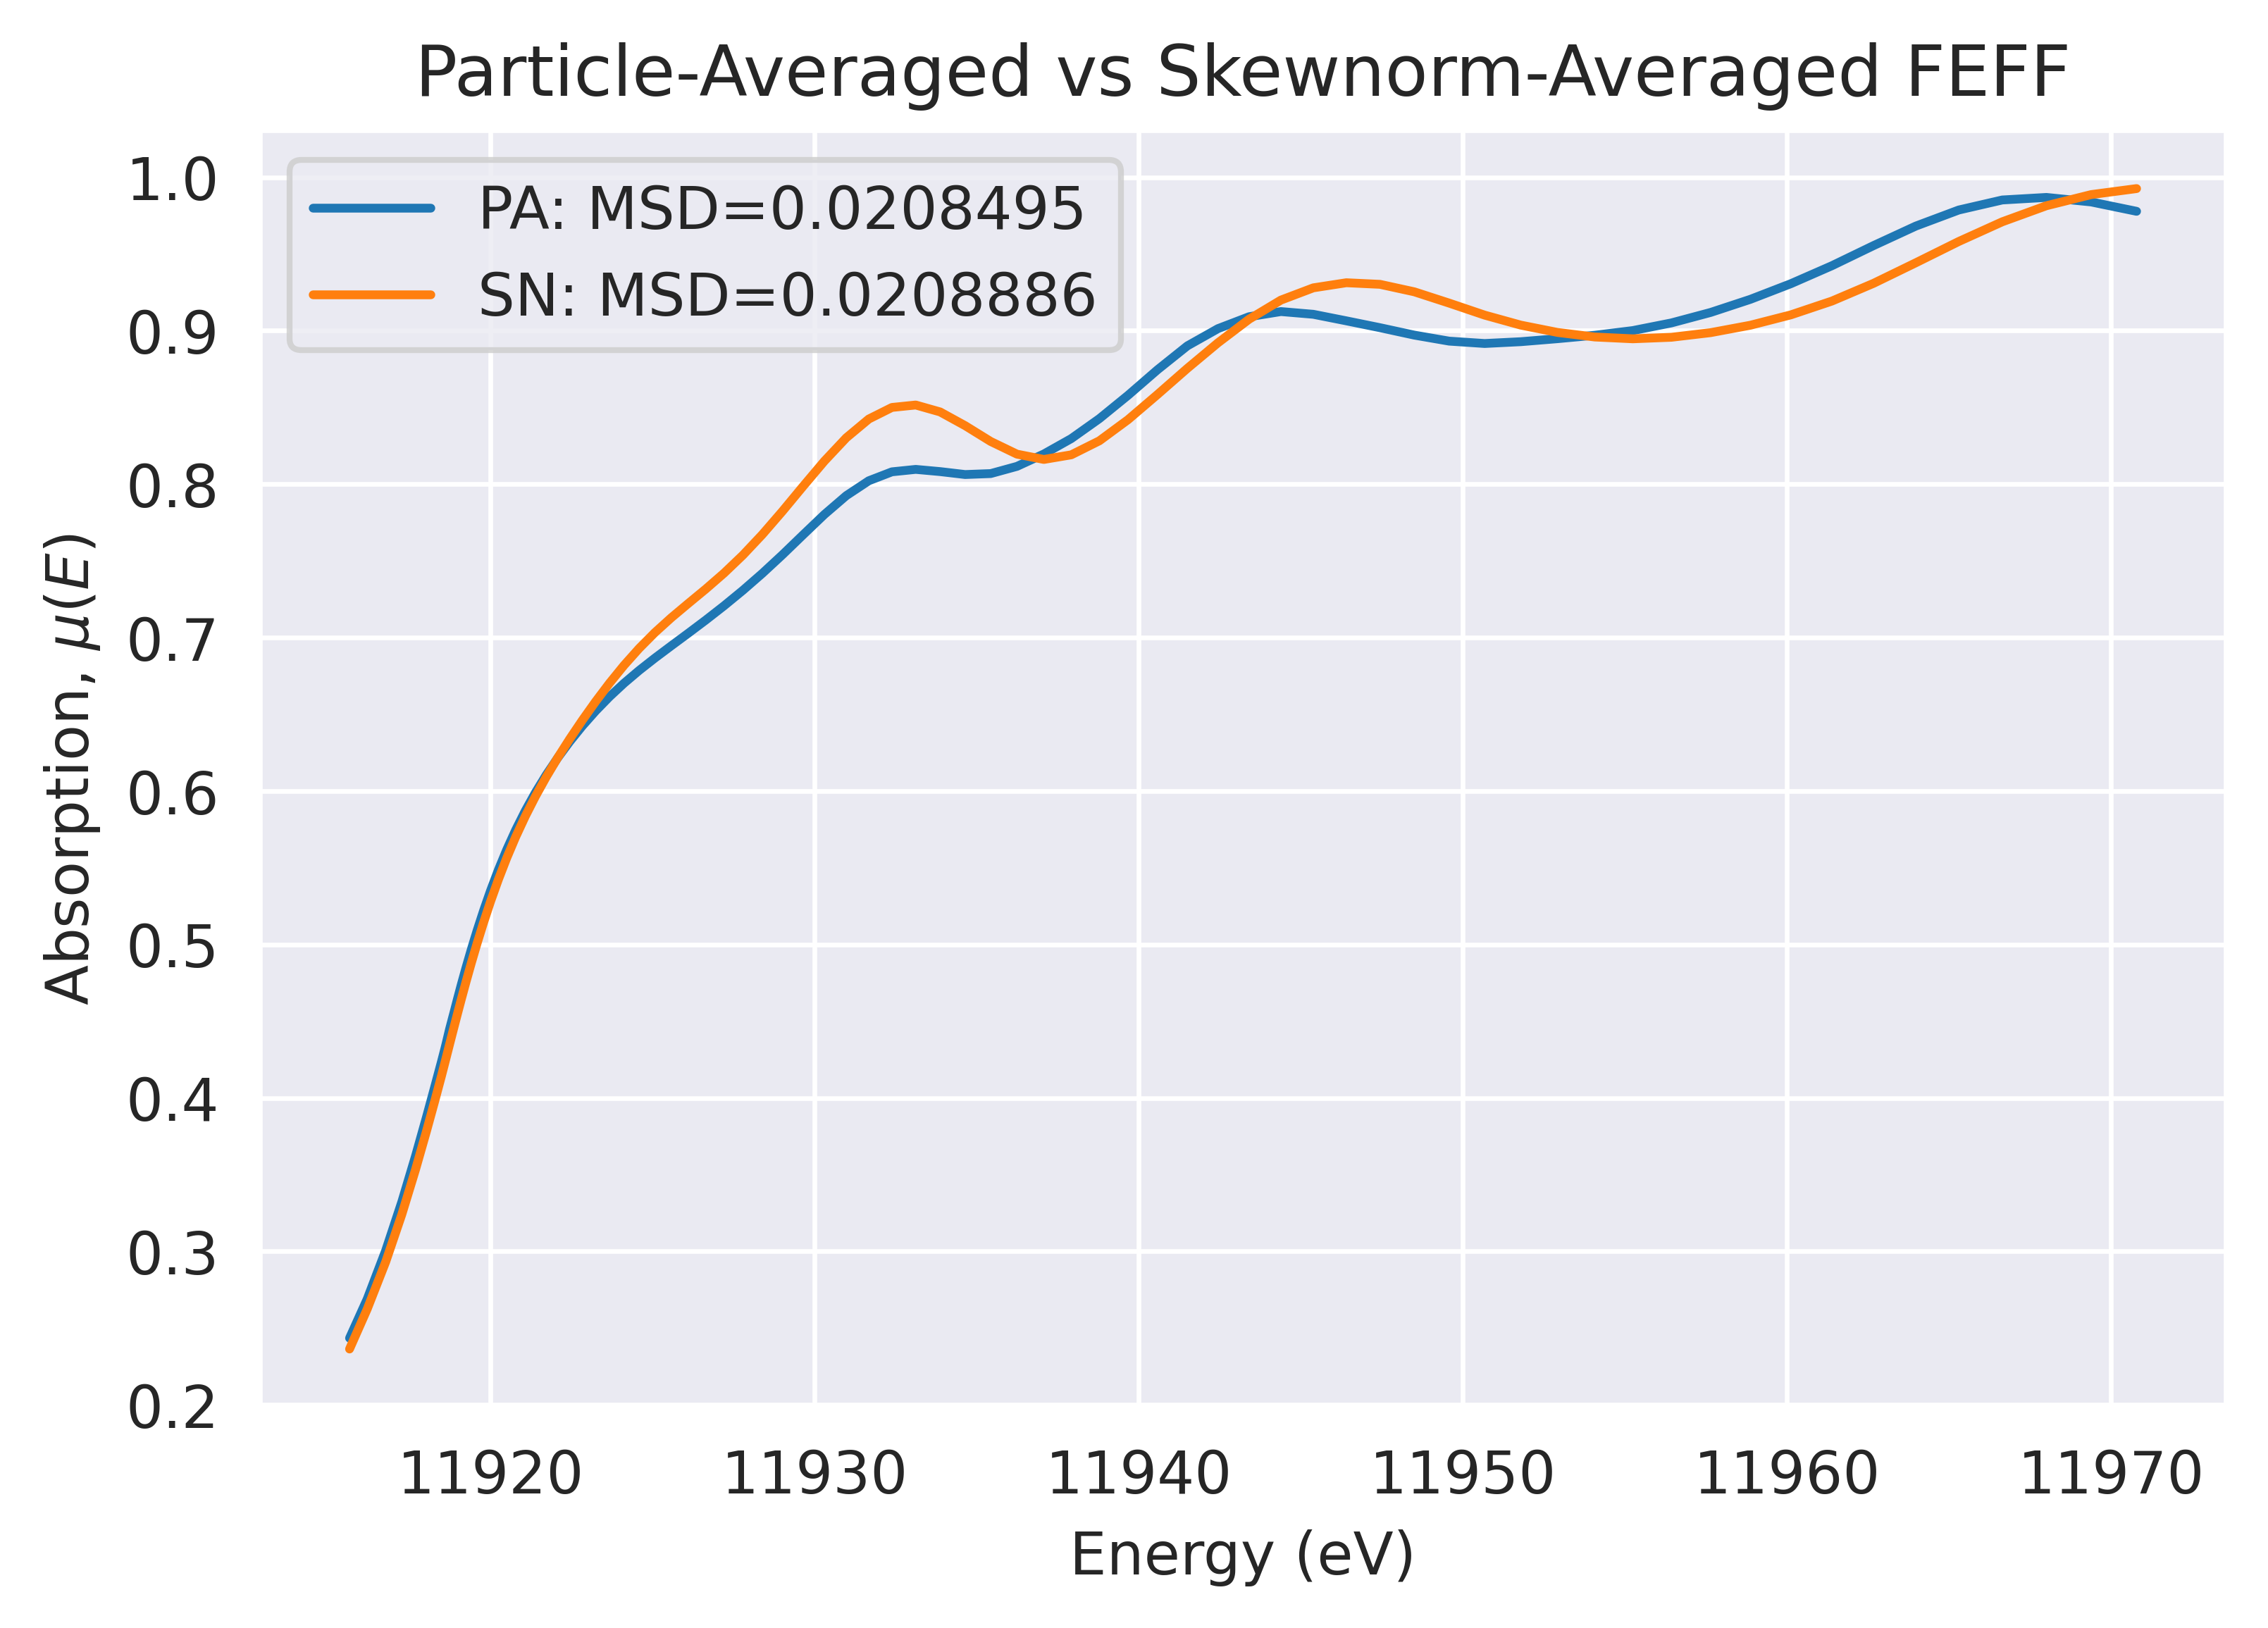
\includegraphics[width=.75\linewidth]{Chapters/Figures/PA-vs-skewnorm-newvals-large-msd.png}
	\caption[Particle-Averaged vs. Skewnorm-Averaged FEFF High-Disorder]{The particle Averaged FEFF vs. Skewnorm Averaged FEFF for particles of high disorder. The systematic differences between the particle averaged feff and the statistical averaged methods are less significant for particles of high-disorder. The persistent differences, however, suggest a false assumption in the statistical averaging mothodology.}
\end{figure}

